\documentclass[article,linenumbers]{agujournal2018}
\usepackage{apacite}
\usepackage{url} %this package should fix any errors with URLs in refs.
\usepackage{amsmath}
\usepackage{ulem}

% Trackchanges package
\usepackage{trackchanges}
\soulregister\ref7
\soulregister\cite7
%% PLEASE USE THE FOLLOWING COMMANDS
%   \note[editor]{The note} 
%   \annote[editor]{Text to annotate}{The note} 
%   \add[editor]{Text to add} 
%   \remove[editor]{Text to remove} 
%   \change[editor]{Text to remove}{Text to add}

% The FIXME macro
\newcommand{\fixme}[1]{\color{red}$<$\textbf{#1}$>$\color{black}}
% The AUTHOR response macro
\newcommand{\rep}[1]{\color{blue}$<$\textbf{AUTHORS}: \textit{#1}$>$\color{black}\\}

%\draftfalse

\journalname{Global Biochemical Cycles}

\begin{document}
	
	%% ------------------------------------------------------------------------ %%
	%
	%  TITLE
	%
	%% ------------------------------------------------------------------------ %%
	\title{Size-differentiated Export in Different Dynamical Regimes in the Ocean}
	
	%% ------------------------------------------------------------------------ %%
	%
	%  AUTHORS AND AFFILIATIONS
	%
	%% ------------------------------------------------------------------------ %%
	\authors{M. Dever\affil{1}, D. Nicholson\affil{1}, M. M. Omand\affil{2}, and A. Mahadevan\affil{1}}
	\affiliation{1}{Woods Hole Oceanographic Institution, Woods Hole, MA 02543, USA}
	\affiliation{2}{Graduate School of Oceanography, University of Rhode Island, Narragansett, Rhode Island, USA}
	
	\correspondingauthor{Mathieu Dever}{mdever@whoi.edu}
	%% ------------------------------------------------------------------------ %%
	%
	%  KEYPOINTS
	%
	%% ------------------------------------------------------------------------ %%
	
	\begin{keypoints}
		\item Submesoscale dynamics enhance the contribution of slow-sinking particles to POC export, especially for steep particle size-spectrum slopes
		\item Remineralization processes intensify the role of slow-sinking particles, to the point where these particle sometime dominate POC export
	\end{keypoints}
	
	%% ------------------------------------------------------------------------ %%
	%
	%  ABSTRACT
	%
	%% ------------------------------------------------------------------------ %%
	\begin{abstract}
		Export of Particulate Organic Carbon (POC) is  mainly driven by gravitational sinking. Thus, traditionally, it is thought that larger, faster-sinking particles make up most of the POC export flux. However, this need not be the case in a dynamic oceanic flow field, where the ocean velocity can influence the descent rate of particles. Particles with different settling speeds are released in two process-oriented model simulations of an upper ocean eddying flow to evaluate the impact of (1) ocean dynamics on the respective contribution of the different sinking-velocity classes to POC export, and (2) the particle number size-spectrum slope. The analysis reveals that the leading export mechanism changes from gravitationally-driven to advectively-driven as submesoscale dynamics become more important. The vertical velocity associated with submesoscale dynamics enhances the contribution of slower-sinking particles to POC export\change{. A steeper particle size spectrum, also increases the relative contribution of smaller, slower-sinking particles}{, especially where the relative abundance of small particles is larger, as captured by a steeper particle size-spectrum slope}. \change{Implementing a r}{R}emineralization \remove{scheme} generally decreases the total amount of biomass exported, but its impact is weaker in dynamical regimes where submesoscale dynamics are present and export is advectively-driven. \change{Under specific conditions}{In an advectively-driven export regime}, remineralization processes counter-intuitively enhance the role of slower-sinking particles to the point where these slower-sinking velocity classes dominate the export, therefore challenging the traditional paradigm for POC export. This study demonstrates that slow-sinking particles can be a significant contribution, and at times, even dominate the export flux. 
	\end{abstract}
	
	%% ------------------------------------------------------------------------ %%
	%
	%  BEGIN ARTICLE
	%
	%% ------------------------------------------------------------------------ %%
	\section{Introduction}
	
	Photosynthesis in the sunlit upper ocean and the production of Particulate Organic Carbon (POC) takes up dissolved inorganic carbon and facilitates the uptake of CO$_2$ from the atmosphere. The sinking of POC exports organic carbon from the upper ocean to the interior, leading to the sequestration of carbon \citep{Falkowski_1998} on timescales ranging from days to years depending on the sinking depth and  circulation. Understanding the mechanisms driving the export of POC from the ocean's surface to the interior is therefore crucial to better constrain Earth's carbon budget.
	
	Traditionally, POC export is thought to occur through gravitational sinking and one-dimensional models have been used to describe the sinking POC flux with depth. Particles produced through primary and secondary production in the surface layer that are relatively large and fast-sinking, tend to sink out of the upper surface layer on timescales shorter than the timescale on which the particles get remineralized. It is reasonable to treat POC export as sinking-dominated if the vertical advective velocities in the ocean are weaker than the velocities associated with gravitational sinking. However, Particulate Organic Matter (POM) has a wide range of particle shape, size and type, that result in particle sinking velocities ranging from practically zero, to several hundreds of meters per day. The size spectrum, or number distribution of particle sizes, is usually characterized by a power law with the power ranging between -2 and -4, for which the abundance of small particles is $\mathcal{O}(10^4 - 10^8)$ greater than large particles. The biomass size spectrum, which indicates the distribution of biomass vs. particle size, tends to be flatter and variable in shape \citep{Sheldon_1972} compared to the particle number spectrum, because the volume (and mass) of a particle scales with its linear size raised to a power that exceeds 1 (and typically varies between 2 and 3 depending on shape and porosity).  Importantly, it means that a significant fraction of the particulate biomass is in the small size fraction. Even though the sinking velocity $w_s$ of particles does not perfectly relate to particle size $l$, it is fair to assume  that  $w_s \sim l^n$ (with $n=2$ according to Stokes law, and $1<n<2$ for complex particle shapes). Due to this, as well as the fact that particles of organic matter are not very much greater in their densities than seawater, a significant fraction of the biomass sinks very slowly (at velocities less than tens of meters per day).  When the gravitational sinking velocity of particles is comparable to (or smaller than) the vertical velocities in the flow field, the dynamics of the flow field can impact the trajectories and fate of the POC.  Thus, depending on the flow dynamics, and the fraction of slow-sinking particulate biomass, the sinking of organic matter can be affected by the fluid flow in the ocean.
	
	Recent studies have shown that ocean dynamics can play a role in driving the transport of carbon from the euphotic layer to the ocean interior.  For example, enhanced vertical velocities along the edge of a mesoscale eddy led to a funneling of particles along the eddy's periphery \citep{vanHaren_2006, Waite_2016}.  
	\cite{Omand_2015}  found that submesoscale mixed layer eddies, while contributing to the restratification of a frontal zone, were subducting a large amount of non-sinking POC from the surface productive layer during the onset of the Spring bloom in the subpolar North Atlantic. Advectively subducting plumes or filaments of high oxygen, chlorophyll and small POC (evidenced through backscatter) were detected from a suite of gliders during the North Atlantic Bloom experiment \citep{Alkire_2012}. Using model simulations to capture the process of eddy-driven subduction, \cite{Omand_2015} estimated the downward advective flux of non-sinking POC and parameterized it. \cite{Briggs_2011} quantified the flux of fast-sinking particles consisting largely of diatoms from observations of optical backscatter. But, these estimates did not account for a range of sinking particle velocities.  Typically, particulate organic matter (POM) has a wide spectrum of sinking velocities and in order to understand its fate and export, we need to consider the biomass distribution as a function of the particle sinking velocity spectrum and its interaction with the dynamics of the flow field in the ocean.
	
	A growing body of literature focusing on submesoscale (1-10 km) dynamics is exploring its impact on biogeochemical processes \citep{Levy_2012,Mahadevan_2016}. Submesoscale dynamics, characterized by Rossby numbers of order 1, typically develop in filaments in areas where sharp density fronts exist \citep{Thomas_2013b,Klein_2009,McWilliams_2016}. In this dynamical regime, geostrophic balance breaks down and a secondary ageostrophic circulation develops across the front, capable of generating large vertical velocities on the order of 100 m/day \citep{FoxKemper_2008,Mahadevan_2016}. On the denser side of the front, the vorticity is cyclonic and associated with downwelling velocities, while anticyclonic vorticity and upwelling is expected on the lighter side of the front. The distribution of relative vorticity across a front is asymmetric and skewed toward cyclonic vorticity \citep{Rudnick_2001}, leading to more localized and more intense downwelling regions, as opposed to weaker and larger upwelling regions \citep{Mahadevan_2006}. Enhanced vertical velocities can generate a local bloom by supplying nutrients to the sunlit layer of the ocean \citep{Mahadevan_2000,Levy_2001}, or can significantly increase the export of POC to the ocean interior through downwelling \citep{Levy_2012, Gruber_2011,Estapa_2015,Omand_2015}.
	
	The downwelling velocities $\mathcal{O}$(100 m/day) generated at submeso-scales provide a physical mechanism capable of competing with gravitational sinking and thus exporting particles over a larger portion of the particle size spectrum. Through this mechanism, smaller particles can be exported on timescales shorter than their remineralization timescales, despite their slower sinking velocities.   Depending on the fraction of  biomass in smaller particles (i.e., with slow sinking velocities), the impact of submesoscale dynamics on the export of POC is potentially significant.
	
	In this study, we account for a range of particle sinking velocities in a dynamic flow field. Despite progress on sampling and viewing particles in the ocean \citep{McDonnell_2010}, direct measurements of particles sinking velocities are difficult to obtain, and often inferred from key parameters such as particle type, size, and density. Though we acknowledge a large variability in these relationships, we assume a relationship between particle size, biomass, and particle sinking velocity in order to assess the impact of the flow dynamics and particle size spectrum on the export flux. 
	
	We  rely on a submesoscale-resolving, non-hydrostatic ocean model to simulate the dynamics in the upper few hundred meters of the ocean. The model does not represent surface waves or boundary layer turbulence, but rather, examines the fate of particulate organic matter beneath the turbulent surface boundary layer.
	The dynamical model is coupled with a particle-tracking module to model the advection of particles by fluid flow, while neglecting the effects of particle inertia and drag on their advection. In addition, the particles sink with a range of sinking velocities (between 0.025--5 m day$^{-1}$) \add{scaled from the range of vertical currents modeled in this region. We aim to address the transitional regime of the particle sinking velocity spectrum, where both advection and sinking speeds have similar order of magnitudes. This transitional regime will thus vary depending on the local dynamics: in strong frontal regions such as western boundary current, vertical currents can $\mathcal{O}$(100 m/day).}
	
	The model is used to quantify the contribution of slow-sinking particles to carbon export, as a function of (1) the dynamics of the flow field, (2) the slope of the sinking velocity spectrum, and (3) the remineralization timescale. Particles in the model are prescribed with both a constant and time-varying sinking velocity to mimic a remineralizing behavior. Particles are released in two fundamentally different flow fields in terms of dynamics based on observed conditions in the Northeast Pacific: In the summer, where ocean dynamics are characterized by low Rossby numbers and weak vertical advective velocities, and in the winter, where ocean dynamics include submesoscale frontal structures and local Rossby numbers $\mathcal{O}$(1). Both simulations and the particle-tracking module are described in Section \ref{sec: Methods}. The impact of particles characteristics and ocean dynamics on the export of POC is quantified in Section \ref{sec: Results}, and discussed in Section \ref{sec: Discussion}. Section \ref{sec: Conclusions} summarizes the key conclusions of the study.
	
	\section{Methods}
	\label{sec: Methods}
	\subsection{Model setup and domain}
	
	This study uses a non-hydrostatic, three-dimensional, Process Study Ocean Model \citep[PSOM;][]{Mahadevan_1996a,Mahadevan_1996b} to simulate an eddy field that is representative of the Northeast Pacific Ocean. The model is set in a channel configuration with periodic east-west boundaries, and solid boundaries in the south and north. The domain covers 112 km in the x-direction, 304 km in the y-direction, and 1000 m in the vertical (Figure \ref{fig: model_domain}). The horizontal resolution is 500 m, while a stretched grid is used in the vertical with 32 levels ranging in thickness from 1.25 m near the surface to 70 m at the lowermost level. The model is integrated numerically in time and evolves the temperature, salinity, free-surface height, pressure, and three-dimensional velocity field from an initial state, subject to momentum and buoyancy fluxes applied through the surface boundary.
	
	% FIG1
	\begin{figure}[ht]
		\centering
		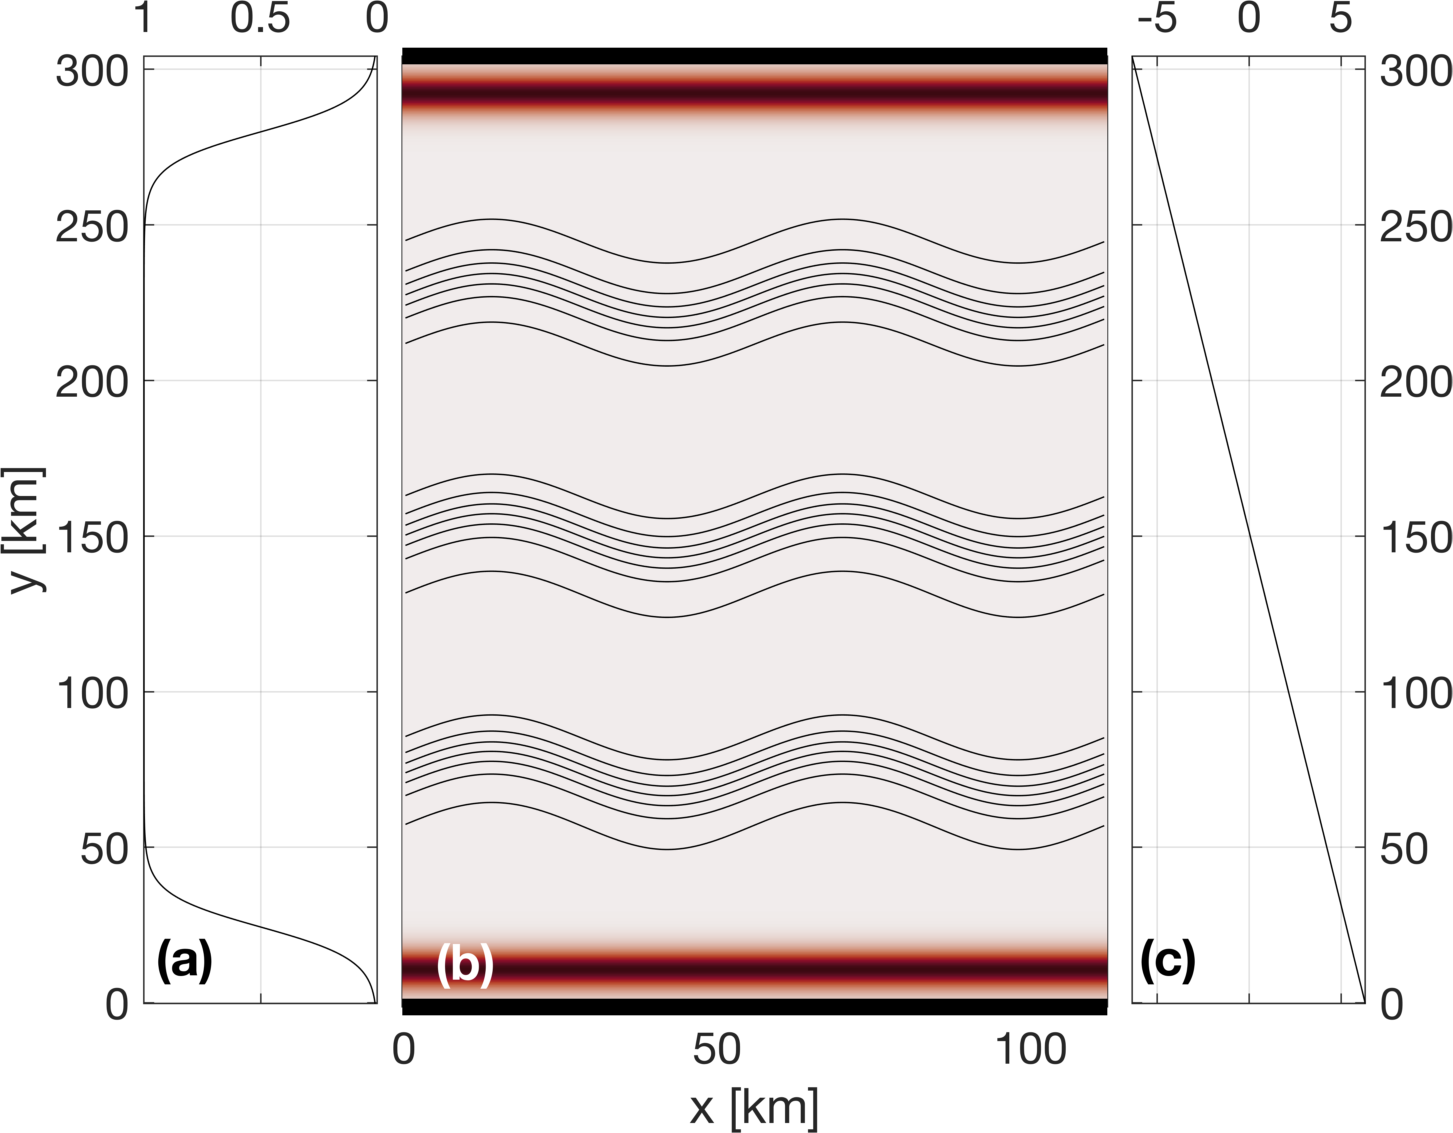
\includegraphics[width = .6\linewidth]{Fig1_model_domain}
		\caption{PSOM model setup. (a) Meridional profile of scaling coefficient that multiplies the time-varying zonal wind stress $\tau_x$ shown in Fig.~3a. The taper at north and south boundaries prevents `coastal' up-/down-welling being entirely concentrated in the boundary grid cell. (b) Restoration factor (color shading) used to dampen internal wave reflection at boundaries as well as up-/down-welling due to the windstress curl. Surface density contours (black) show the three fronts used to initialize the model. (c) Meridional variation of the time-dependent surface  heat flux (Fig.~3a) prescribed over the domain.}
		\label{fig: model_domain}
	\end{figure}
	
	Time-varying wind stress and heat flux are prescribed at the surface boundary. Time series are computed from measurements collected at Station Papa and available through the Pacific Marine Environmental Laboratory \citep{PMEL_data}. Daily wind stress and net heat fluxes are calculated over the period 2007-2016 to produce a year-long climatology. A squared low-pass filter with a cut-off frequency of 8.5 days is applied to both time series to remove high-frequency variability. In all numerical experiments, simulations are 
	run for the first 5 days without any forcing applied to the surface boundary. Surface wind stress and heat fluxes are then linearly ramped up between days 5 and 10 of the simulation, to reach realistic values at day 10.
	
	While the meridional component, $\tau_y$, is set to zero, the zonal component of the wind stress, $\tau_x$, is prescribed at the surface throughout the model domain and is tapered at the northern and southern boundaries to avoid excessive Ekman-driven upwelling and downwelling (Figure \ref{fig: model_domain}a). A restoration timescale is prescribed to contain the curl-driven upwelling and downwelling regions generated by the tapering of the wind stress, as well as to limit internal wave reflection at the solid boundaries back into the domain (Figure \ref{fig: model_domain}b). While net surface heat fluxes are homogeneous in the zonal direction, a meridional gradient is maintained throughout the simulation. The meridional gradient was determined from the North American Regional Reanalysis (NARR) product \citep{Mesinger_2006}, and set to 1/24 W/m$^2$/km (Figure \ref{fig: model_domain}c).
	
	Initial hydrographic conditions are determined from a three-dimensional gridded field of temperature and salinity from Argo floats \citep{Gaillard_2015,Gaillard_2016}. Argo data is averaged monthly over the period 2002-2012 and two different months are used to initialize the two main numerical experiments for this study: Climatological conditions in April are used to initialize the \textit{Papa\_summer} experiment, while January climatological conditions are used to initialize the \textit{Papa\_winter} experiment (Table \ref{tab: meso_vs_submeso}). The north-south background density gradient is then intensified into three fronts located at $y = 75$, $y = 150$, and $y = 225$ km (Figure \ref{fig: model_domain}). The amplitude of the density gradient associated with the three fronts is determined from the probability distribution function (PDF) of the density gradients measured by underwater gliders deployed around Station Papa over the period 2008-2010 \citep{Pelland_2016,Pelland_2018_data}. To reduce model spin-up time, density fronts are perturbed by a sinusoidal wave with a wavelength close to the 1st baroclinic deformation radius ($\lambda = $ 66 km). Similar PSOM configurations were successfully used in previous studies \citep{Mahadevan_2012,Omand_2015}.
	
	Two main experiments are conducted using the same configuration of PSOM, where only initial conditions and surface forcings are varied: \textit{Papa\_summer} aims at generating ocean dynamics representing conditions in the Northeast Pacific in the summertime. Summer ocean dynamics are characterized by a flow generally in geostrophic balance, with relatively weak density gradients and low Rossby numbers ($\ll$1). \textit{Papa\_winter} aims at capturing wintertime ocean conditions in the region. A different dynamical regime is expected to dominate during wintertime when mixed layers are deeper and lateral density gradients enhanced, with sharper density fronts, filament-like features and localized Rossby number $\mathcal{O}$(1) over spatial scales $\mathcal{O}$(1 km) \citep{Mensa_2013,Callies_2015,Thompson_2016}. The individual characteristics of each of \linebreak \textit{Papa\_summer} and \textit{Papa\_winter} are detailed below.
	
	\subsubsection{\textit{Papa\_summer} Model Experiment}
	
	In \textit{Papa\_summer}, PSOM is initialized based on climatological Argo data in April. The magnitude of the density gradient across the front is set to 3.34$\times$10$^{-6}$ kg/m$^3$/m, which corresponds to the 95$^{th}$ percentile of the PDF of density gradients measured in April from glider data collected in the region (Figure \ref{fig: Papa_summer} and Table \ref{tab: meso_vs_submeso}). The model is run with a timestep of 216 s and is allowed to spin-up for 60 days, allowing summer stratification to develop. The model is then run for 30 additional days, saving instantaneous model fields every 3 hours for particle tracking. The month of April is chosen for initialization so the experiment would capture the onset of positive net heat fluxes, and the summer restratification that ensues in July-August (Figure \ref{fig: Papa_summer}). In this region, the summer stratification is associated with large primary productivity, particle production, and POC export \citep[e.g., fecal pellets, dead phytoplankter; ][]{Plant_2016}.
	
	%TAB1
	\begin{table}[t]
		\caption{Summary of the key characteristics of PSOM experiments \textit{Papa\_summer} and \textit{Papa\_winter}.}
		\label{tab: meso_vs_submeso}
		\centering
		\centering
		\begin{tabular}{|l|c|c|}
			\hline
			& \textit{Papa\_summer} & \textit{Papa\_winter} \\
			\hline
			Time period 								& April -- July             & January -- March          \\
			Spin-up								        & 60 days                   & 50 days                   \\
			Advective timestep				            & 216 s                     & 108 s                     \\
			Horizontal diffusivity			            & 1 m$^2$ s$^{-1}$          & 0.2 m$^2$ s$^{-1}$        \\
			Restoration timescale			            & 3 days                    & 15 days                   \\
			Zonal wind stress                	        & 0 -- +0.16 N m$^{-2}$      & -0.05 -- +0.17 N m$^{-2}$  \\	
			Surface heat flux               	        & -46.8 -- +167.5 W m$^{-2}$ & -57.6 -- +15.3 W m$^{-2}$  \\
			Maximum M$^2$ ($\times$10$^{-8}$)	        &                           &                           \\
			\multicolumn{1}{|r|}{initial}	            & 3.2 s$^{-2}$              & 33.9 s$^{-2}$             \\
			\multicolumn{1}{|r|}{spun-up}	            & 12.0 s$^{-2}$             & 50.0 s$^{-2}$             \\	
			Maximum N$^2$ ($\times$10$^{-4}$)	        &                           &                           \\
			\multicolumn{1}{|r|}{initial}	            & 1.5 s$^{-2}$              & 1.6 s$^{-2}$              \\
			\multicolumn{1}{|r|}{spun-up}	            & 3.1 s$^{-2}$              & 1.1 s$^{-2}$              \\	
			Averaged mixed layer depth                  &                           &                           \\
			\multicolumn{1}{|r|}{initial}	            & 73 m                      & 85 m                      \\
			\multicolumn{1}{|r|}{spun-up}	            & 11 m                      & 93 m                      \\	
			\hline
		\end{tabular}
	\end{table}
	
	% FIG2
	\begin{figure}[t]
		\includegraphics[width = 1\linewidth]{Fig2_Papa500_summer}
		\caption{PSOM configuration for \textit{Papa\_summer}. (a) Time series of net heat fluxes and wind stress prescribed at the surface. Notice the positive heat fluxes, as well as downfront winds (i.e. eastward) persisting throughout the experiment. (b)-(d) surface horizontal buoyancy gradients $M^2 = |\nabla_Hb|^2$ (in s$^{-2}$) at day of year (doy) 105, 135, and 165. Black contours show isopycnals (in kg/m$^3$; CI = 0.01 kg/m$^3$). (e) Vertical profile of the buoyancy frequency $N^2$ at day of year 105, 135, 165, and 195, showing the development of summer stratification centered at z = 30 m (solid lines). Monthly-average vertical stratification obtained from glider profiles collected in June and July are superimposed (dashed lines), along with the correlation coefficient between observations and model outputs.}
		\label{fig: Papa_summer}
	\end{figure} 
	
	
	\subsubsection{\textit{Papa\_winter} Model Experiment}
	
	In \textit{Papa\_winter}, PSOM is initialized based on climatological Argo data in January. The frontal gradient is set to 3.54$\times$10$^{-5}$ kg/m$^3$/m, which corresponds to the 99$^{th}$ percentile of the PDF of density gradients measured in January from glider data collected in the region (Figure \ref{fig: Papa_winter} and Table \ref{tab: meso_vs_submeso}). The model is allowed to spin-up for 50 days allowing for the prescribed fronts to become unstable. To accommodate for the larger density gradients and stronger velocities, the advective timestep is shortened to 108 s and the horizontal diffusivity is lowered to 0.2 m$^2$/s throughout the experiment. The model is run for 30 additional days, saving instantaneous model fields every 1.5 hours for particle tracking. The month of January is chosen for initialization so the experiment would capture the time of year where the mixed layer is the deepest, and Rossby number O(1) occur more frequently. The objective is for this experiment to contrast \textit{Papa\_summer} by capturing the statistics of ocean conditions dominated by submesoscale dynamics.
	
	% FIG3
	\begin{figure}[ht]
		\includegraphics[width = 1\linewidth]{Fig3_Papa500_winter}
		\caption{PSOM configuration for \textit{Papa\_winter}. (a) time series of net heat fluxes and wind stress prescribed at the surface. Notice the mostly negative heat fluxes, as well as alternating zonal wind direction. (b)-(d) surface horizontal buoyancy gradients $M^2 = |\nabla_Hb|^2$ (in s$^{-2}$) at day of year (doy) 0, 30, and 50. Black contours show isopycnals (in kg/m$^3$; CI = 0.01 kg/m$^3$). (e) Vertical profile of the buoyancy frequency $N^2$ at doy 0, 30, 50, and 80, showing the persistence of the halocline between z = 80 and z =180 m throughout the experiment (solid lines). Monthly-average vertical stratification obtained from glider profiles collected in March is superimposed (dashed line), along with the correlation coefficient between observations and model outputs.}
		\label{fig: Papa_winter}
	\end{figure}
	
	
	\subsubsection{Validation}
	\label{sec: glider_validation}
	
	To ensure that PSOM simulations yielded realistic conditions for both \textit{Papa\_summer} and \textit{Papa\_winter}, distributions of horizontal ($M^2$) and vertical ($N^2$) buoyancy gradients are compared with glider observations collected over the period 2008-2009 \citep{Pelland_2016}.
	During this period, underwater gliders sampled in a ``bow-tie" pattern centered on Station Papa. Gliders sample the water column in a triangular wave pattern, whose shape is easily affected by currents, due to the slow moving speed of the glider ($\sim$1 km/hr). It is therefore challenging to associate a specific spatial scale with gradients computed between glider profiles, as profile separation distances can be highly variable through depth and time. To circumvent this issue, horizontal buoyancy gradients are computed between each pair of glider profiles available within one branch of the bow-tie. Each along-track lateral buoyancy gradient is thus associated with a specific separation scale and a timestamp. Glider-based density gradients can be affected by internal waves. To filter the impact of internal waves on the PDF of horizontal buoyancy gradients, only gradients computed at a scale of twice the Rossby radius $\pm$ 1 km are considered. Rossby radii are estimated from the glider data and are $\sim8$ km in winter and $\sim20$ km in summer.
	
	\subsection{Particle Tracking Experiments}
	
	\subsubsection{Particle Advective Scheme}
	To quantify the impact of submesoscale dynamics on the export of Particulate Organic Matter (POC), Lagrangian particle trajectories are computed using the same scheme as in ``TRACMASS'' \citep{Doos_2013} with the flow fields from the two experiments described above. The three-dimensional, non-divergent velocity components from the faces of each ``C" grid cell are linearly interpolated onto the particle's position within the grid cell. For example, the eastward (along the x-axis) velocity  of a particle is given by
	\begin{equation}
		u(x) = u_{i-1} + \frac{(x - x_{i-1})}{(x_i - x_{i-1})}(u_{i}-u_{i-1}),
	\end{equation}
	where the subscripts $i-1$ and $i$ denote the western and eastern walls of the grid cell where the particle is located, respectively. This can be re-written as
	\begin{equation}
		\frac{\partial x}{\partial t} + \beta x + \delta =  0,
		\label{eq: eq_diff}
	\end{equation}
	where $\beta = (u_{i}-u_{i-1})/\Delta x$ and $\delta = -u_{i-1} - \beta x_{i-1}$ \citep{Doos_2013}. This differential equation can be solved analytically for $\beta \neq 0$ as
	\begin{equation}
		x_{t_1} = \left(x_0 + \frac{\delta}{\beta}\right)\exp^{-\beta(t_1 - t_0)} - \frac{\delta}{\beta}
		\label{eq: PT_advection}
	\end{equation}
	The time it will take for the particle to reach the eastern or western face of the grid cell can be computed by taking $x_{t_1} = x_i$ or $x_{t_1} = x_{i-1}$, respectively, and solving for $t_1$. For each advective timestep, the times required for the particle to reach any of the 6 walls of the grid cell are computed using (\ref{eq: PT_advection}). If any of those times is shorter than the advective timestep, the particle is advected until it reaches the cell wall. Then the flow field in the adjacent grid cell is considered and the particle is advected over the remaining time. 
	
	\subsubsection{Particle Seeding}
	
	For all particle-tracking experiments, a single particle seeding event is prescribed. In the horizontal, particles are seeded every 250 m over the entire domain in the x-direction, and for 100 $<y<$ 200 km in the y-direction. The seeding is centered over the mean position of the central front (see Figure \ref{fig: Papa_summer}) and is therefore not affected by undesired effects created by the solid north-south solid boundaries. In the vertical, particles are seeded every 1 m between 75 and 85 m. This depth range is chosen as it corresponds to the average euphotic depth at Station Papa, defined by the 1\% light level. \add{Particle seeding is located at the base of the euphotic layer where biological processes not captured by the particles (e.g., grazing, repackaging, aggregation, etc.) are not as active }\citep{Duclow_2001}.
	The euphotic depth was computed for the months of February and June over the period 2007-2016 from profiles of Photosynthetically \change{Available}{Active} Radiation (PAR) collected at Station Papa as part of the long-term monitoring of Line P executed by the Department of Fisheries and Ocean Canada\footnote{https://www.waterproperties.ca/linep/index.php}. The average euphotic depth computed for both of these months is around 80 m, which agrees with previously established estimates of the euphotic depth \citep{Sherry_1999,Harrison_2004}.
	
	In each particle-tracking experiment, four different classes of particles are released. Each particle class is characterized by a different sinking velocity: 0.025, \remove{0.05, }1, and 5 m/day. \add{In this study, these particle classes are refered to as slow- intermediate-, and fast-sinking particles. This characterization is not based on the absolute value of the sinking rate, but rather on the ratio with vertical currents in the study region.} While 5 m/day remains a relatively slow sinking rate, } The slowest-sinking class is essentially selected to represent non-sinking particles: based on the setup of our experiments, the slowest-sinking particles would take 800 days on average to be exported to a depth of 100 m through gravitational sinking, a timescale much greater than commonly observed remineralization timescales. The fastest-sinking velocity is chosen as an end-member velocity class of particle\change{ that will be exported in its entirety over the course of our experiment. }{, based on the PDF of vertical velocities in the model. At any given time, at least 85\% of the model vertical velocity is weaker than 5 m/day. The results presented for the 5 m/day sinking class can therefore be theoretically extrapolated to any class with a higher sinking velocity.}
	
	The advective timestep for particles is set to 1.5 hours. The flow field is linearly interpolated in time between model outputs, justifying the higher temporal resolution used for particle tracking in \textit{Papa\_winter}. Particle positions are saved every 3 hours, along with key model variables interpolated onto the particle positions (e.g., density, vorticity). Particles are tracked for \change{three}{four} weeks (28 days). Each particle-tracking experiment contains 1,971,717 particles per sinking-velocity class, for a total of 9,858,585 particles. Particles located deeper than the maximum winter mixed layer \citep[i.e., 100 m;][]{Pelland_2016, Plant_2016} are considered exported, as they will likely not be re-entrained into the mixed layer.
	
	\subsubsection{Density and Biomass Spectra}
	\label{sec: equations_biomass}
	The slope $\xi$ of the size spectrum of particles \citep[also know as the Junge slope;][]{White_2015} is the slope of the log-log curve of particle number $N$ vs. particle radius $r$, where
	\begin{equation}
		N(r) = N_0 \left(\frac{r}{r_0}\right)^{-\xi}.
		\label{eq: powerlaw_radius}
	\end{equation}
	Here, $N_0$ and $r_0$ represent a reference particle number and radius, chosen arbitrarily. For small particles ($<$400 $\mu$m) and relatively low temperature ($<$15$^o$C), it has been shown that the relationship between particle radius $r$ and sinking velocity $w_s$ exhibits a range of variation and is difficult to determine empirically. Nevertheless, Stokes' law, where $w_s \propto r^2$, is often used as a lower-bound sinking velocity estimate \citep{Bach_2012}.
	
	Assuming a Stokes-like relationship, we can construct a particle sinking velocity spectrum $N(w_s)$ based on (\ref{eq: powerlaw_radius}), as
	\begin{equation}
		N(w_s) = N_0 \left(\frac{w_s}{w_{s_0}}\right)^{-\xi/2},
		\label{eq: powerlaw_velocity}
	\end{equation}
	where $w_{s_0}$ is the sinking speed of particles with radius $r_0$.
	For a specific slope and sinking-velocity class, an equivalent number of particles per simulated particle can be computed using (\ref{eq: powerlaw_velocity}) (See Figure \ref{fig: sinking_velocity_spectrum}). For example, using the largest sinking velocity class as a reference (i,.e., $w_{s_0} = 5$ m/day and $N_0=$1,971,717), and a spectral slope $\xi = 4$, each simulated particle with a sinking velocity of 0.025 m/day in fact represents 40,000 particles (Figure \ref{fig: sinking_velocity_spectrum}). The relative biomass of a particle in a specific sinking-velocity class, $B_p(w_s)$ can be estimated if the biomass is assumed to scale with the particle's volume. The relative biomass of one particle in a sinking-velocity class $w_s$ can therefore be computed as
	% FIG4
	\begin{figure}[ht]
		\centering
		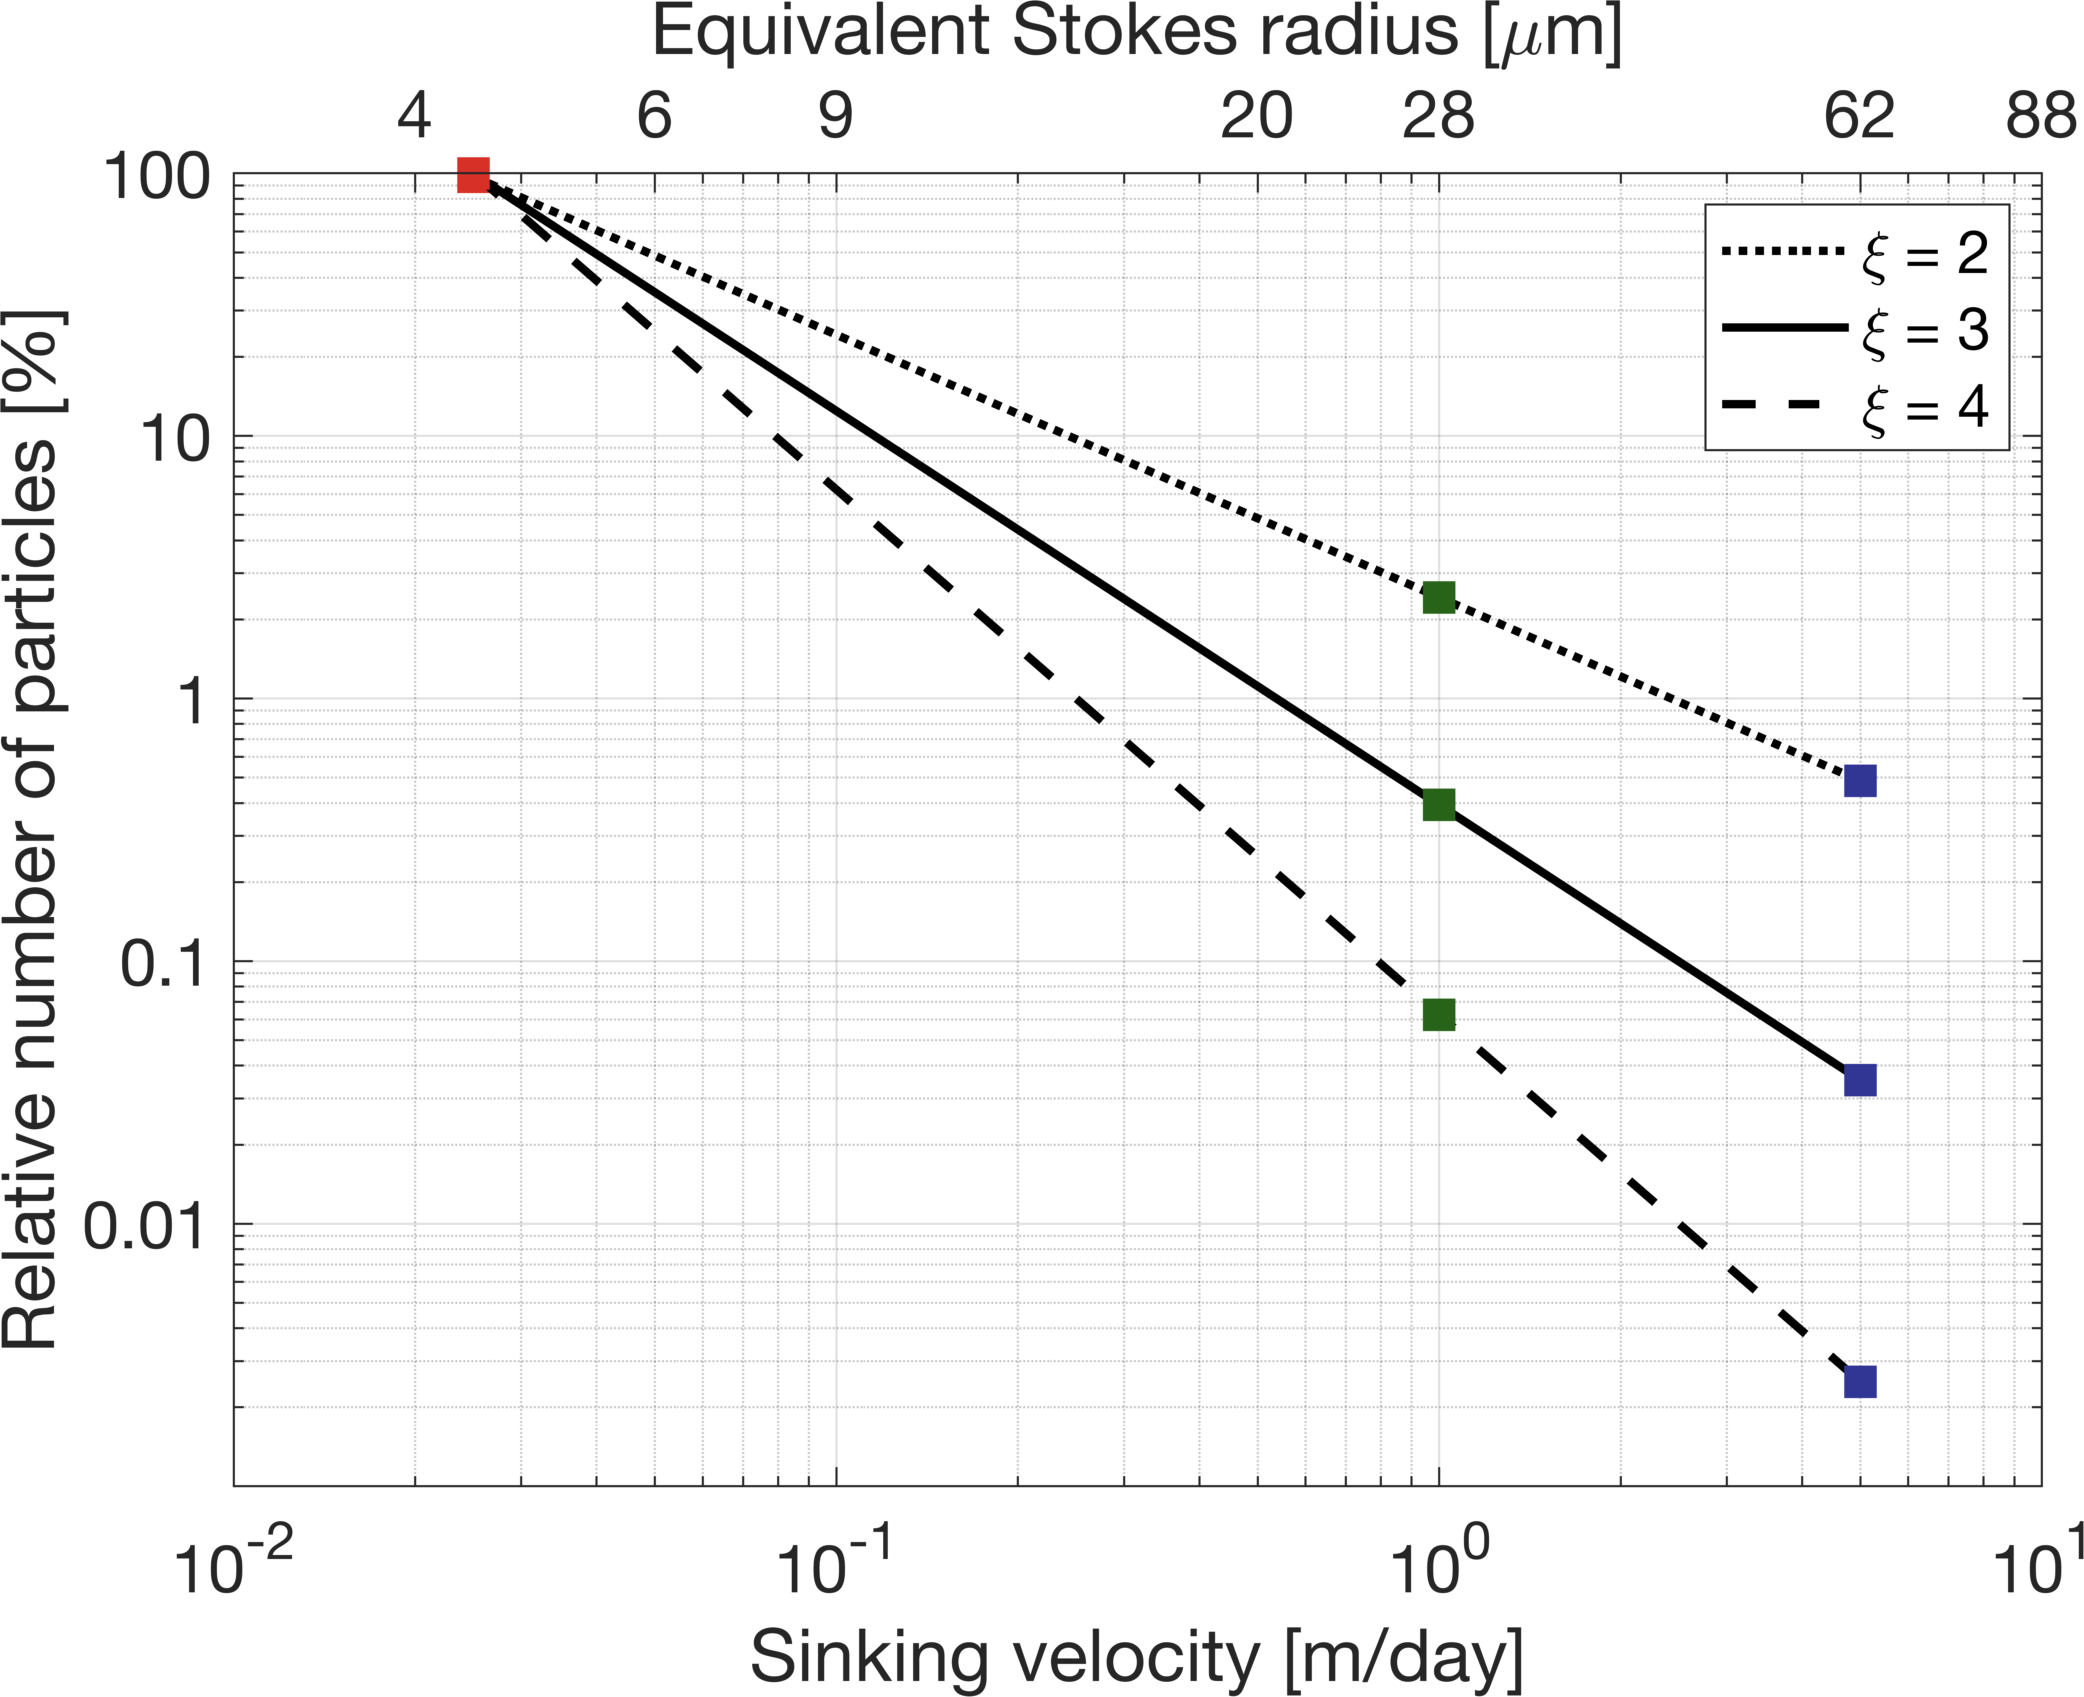
\includegraphics[width = .49\linewidth]{Fig4b.png}
		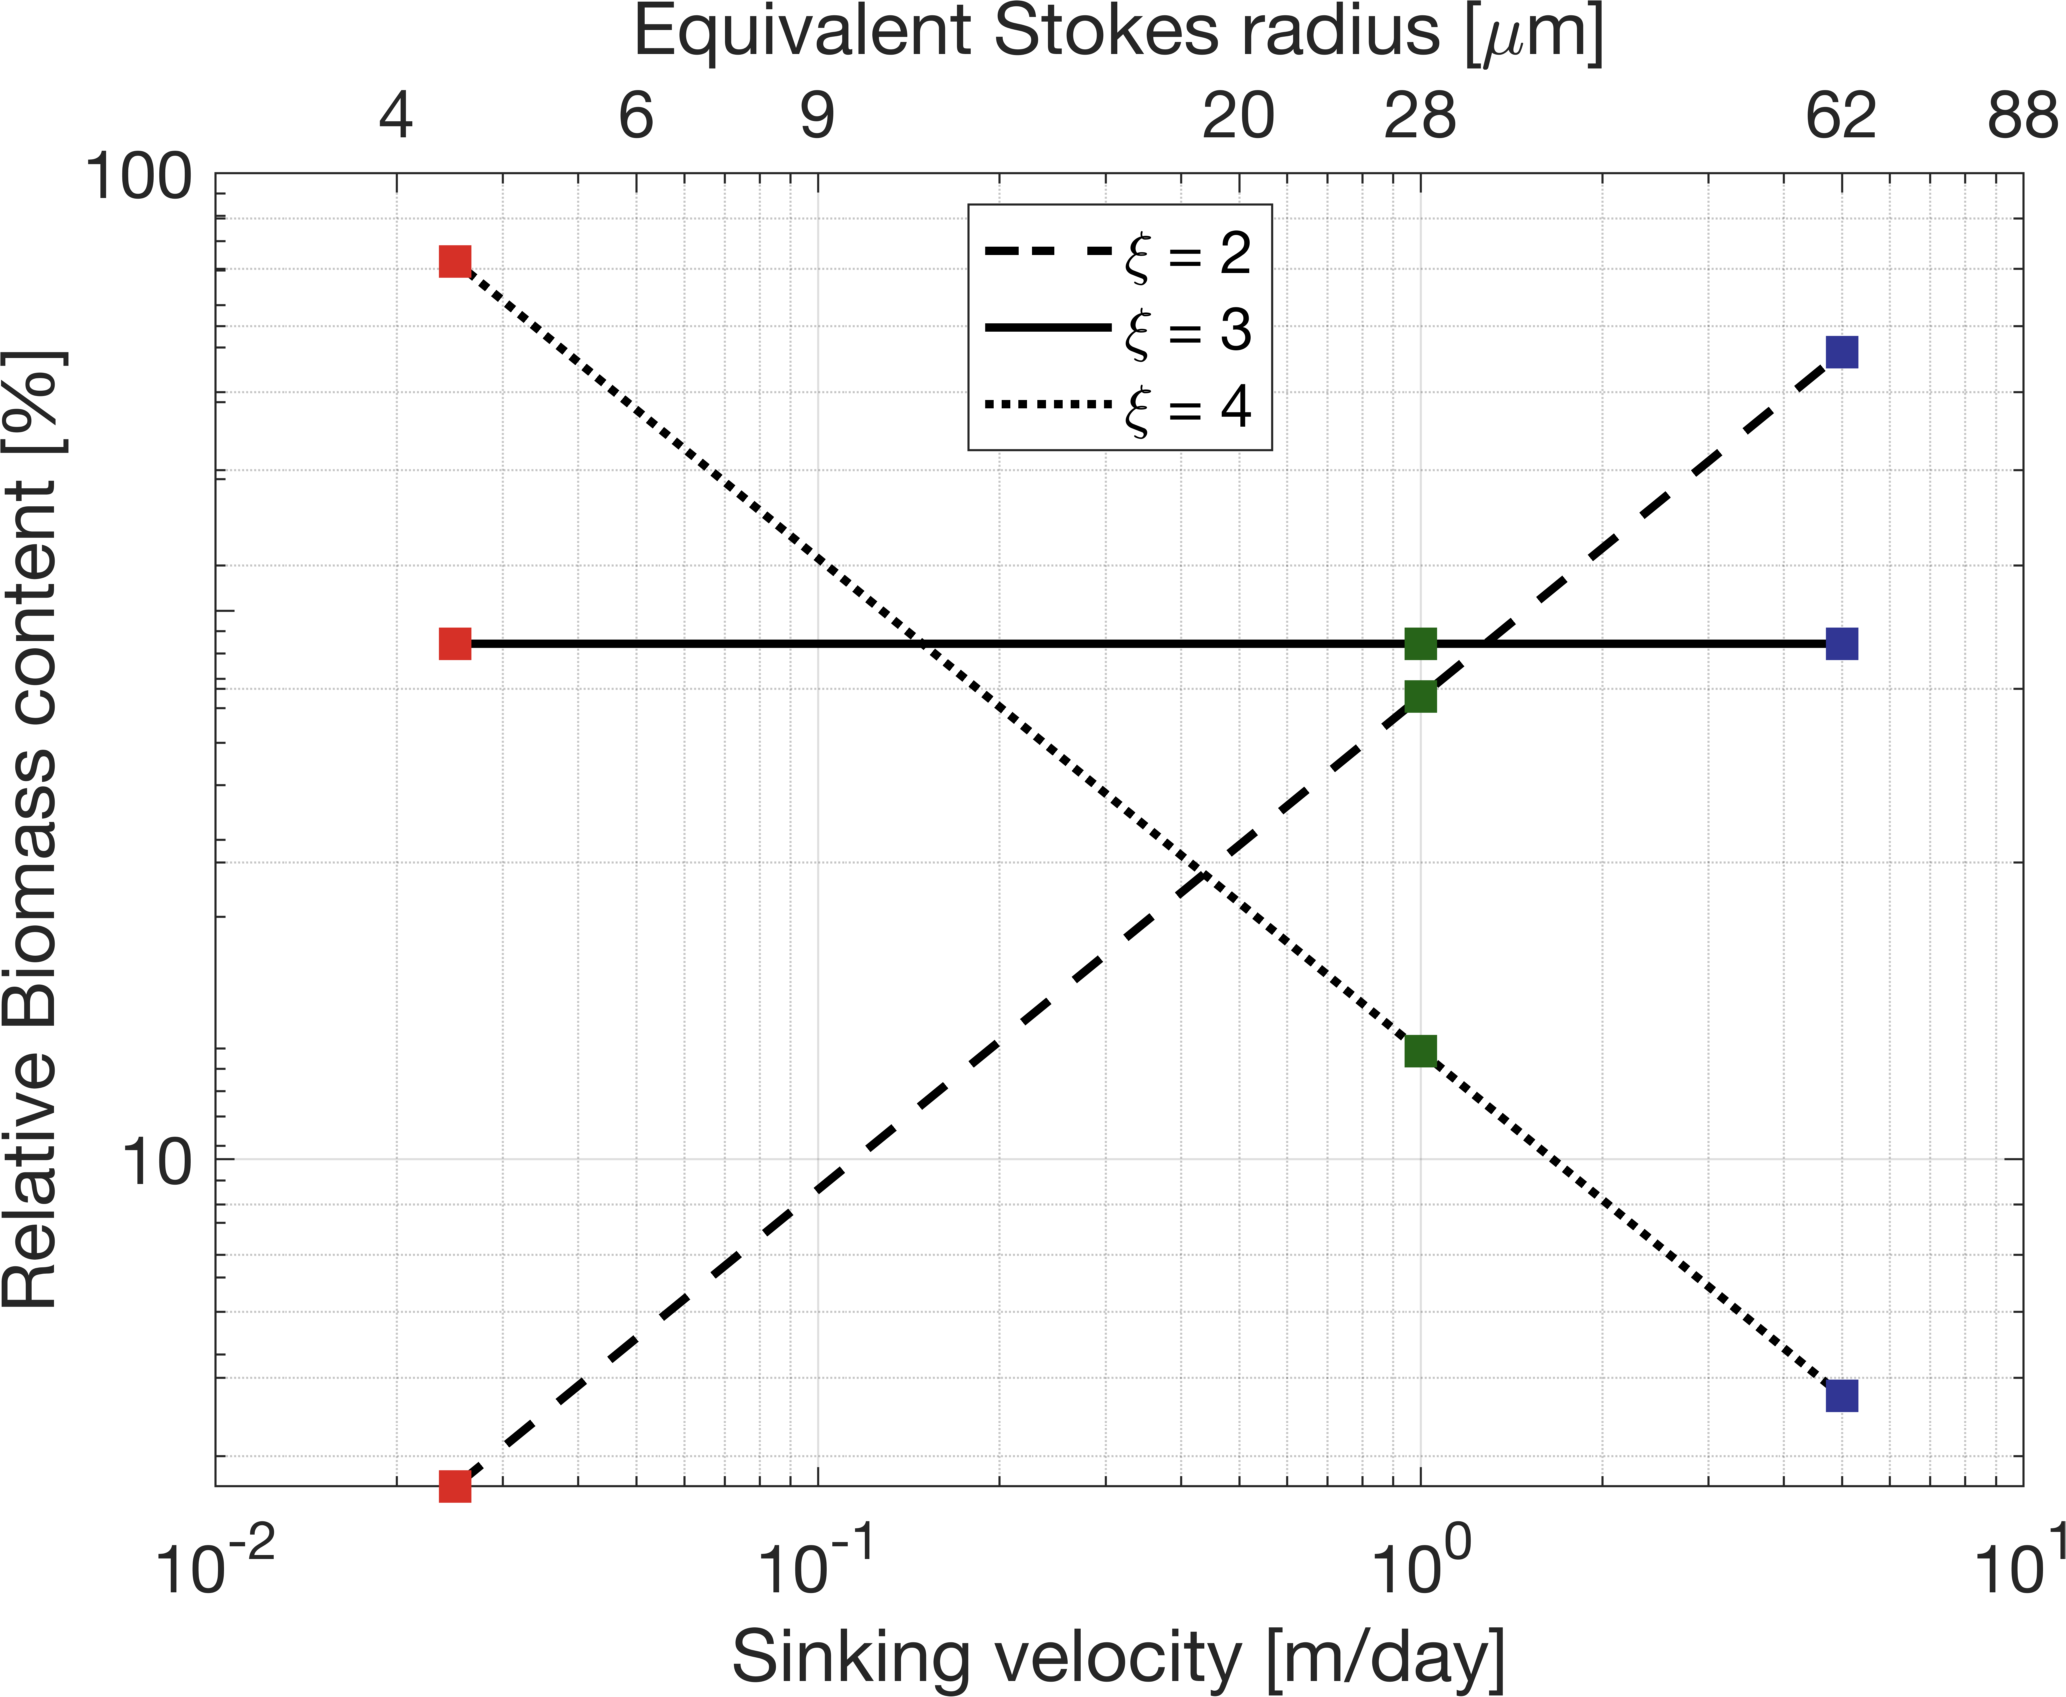
\includegraphics[width = .49\linewidth]{Fig4a.png}
		\caption{Relative number of particles (left) and biomass (right) as a function of sinking velocity $w_s$. Sinking velocity spectrum are shown for three different Junge slope $\xi$: 2 (dotted), 3 (solid), and 2 (dashed). Colored squares indicate the sinking velocities of the three particle classes modeled: 0.025 m/day (red), 1 m/day (green), and 5 m/day (blue).}
		\label{fig: sinking_velocity_spectrum}
	\end{figure}
	\begin{equation}
		B_p(w_s) = B_p(w_{s_0})\left(\frac{w_s}{w_{s_0}}\right)^{3/2}
		\label{eq: biomass_realparticle}
	\end{equation}
	where $B_p(w_{s_0})$ is the biomass of a particle in the sinking velocity class $w_{s_0}$. The total biomass associated with one simulated particle can be obtained by scaling (\ref{eq: biomass_realparticle}) by the ratio $N(w_s)/N_0$:
	\begin{equation}
		B(w_s) =  B_0\left(\frac{w_s}{w_{s_0}}\right)^{3/2}\frac{N(w_s)}{N_0}
		\label{eq: biomass_simulatedparticle}
	\end{equation}
	where $B_0 = B_p(w_{s_0})$. Combining (\ref{eq: powerlaw_velocity}) and (\ref{eq: biomass_simulatedparticle}) yields an expression relating the biomass associated with a simulated particle for a specific sinking-velocity class and the spectral slope (Figure \ref{fig: sinking_velocity_spectrum}):
	\begin{equation}
		B(w_s) = B_0\left(\frac{w_s}{w_{s_0}}\right)^{\frac{3-\xi}{2}}.
		\label{eq: biomassjungeslope}
	\end{equation}
	Using the same example as before where $\xi = 4$, if the amount of biomass associated with one simulated particle in the 5 m/day sinking-velocity class is taken as $B_0 = 1$, then one simulated particle sinking at 0.025 m/day contains 14.14 units of biomass and a single particle contains $14.14/40,000 =3.5\times10^{-4}$ units of biomass (see Figure \ref{fig: sinking_velocity_spectrum}). This normalized formulation of particle number and biomass (see Equations (\ref{eq: powerlaw_velocity}) and (\ref{eq: biomassjungeslope})) has the advantage that the impact of spectral slope on the relative export of biomass can be quantified without needing a large number of particle-tracking experiments, where the number of seeded particles would vary to account for the different spectral slopes. For the purpose of this study, only the relative amount of biomass is relevant. For simplicity, we define a normalized biomass unit for $\xi =3$ as $B_0=$ 1. The values taken by $B_0$ for other Junge slopes $\xi$ are computed under the condition that the total amount of biomass is kept constant (Figure \ref{fig: sinking_velocity_spectrum}b).
	
	\subsubsection{Particle Remineralization Scheme}
	\label{sec: remin_scheme}
	Remineralization of particles as they sink through the water column impacts the amount of biomass exported. Slow-sinking particles generally contain less biomass and spend more time in the mixed layer, which means that they are remineralized at a shallower depth than faster sinking particles. Remineralization processes are complex, species-dependent, and generally not well-understood. In the absence of a consensus on a general functional form of particle remineralization, we rely on an idealized relationship which assumes that the biomass content of a particle decreases in time proportionally to the particle volume. Remineralization is thus modeled as an exponential decrease of biomass with time at a rate $k$ \citep{Iversen_2010, Iversen_2013}
	\begin{equation}
		B (t) = B^0\exp(-kt),
		\label{eq: remin_scheme}
	\end{equation}
	where $B^0$ denotes the biomass content at $t = 0$ days, and the remineralization rate is taken to be $k = 0.13$ day$^{-1}$ in this study \citep{Iversen_2010}. This remineralization rate is independent of particle sinking velocity, and seems to lie within the range of other estimates \citep{Ploug_2008, Iversen_2010, Iversen_2013}. The change in biomass with time is in turn expected to affect the sinking velocity of the particle. Given that $B \propto w^{3/2}$ (see Equation (\ref{eq: biomass_realparticle})), particles in all sinking-velocity classes undergo a decay in sinking speed according to
	\begin{equation}
		w_s (t) = w_s^0\exp(-\frac{2kt}{3}),
		\label{eq: sinking_velocity_remin}
	\end{equation}
	where $w_s^0$ is the initial sinking velocity at $t = 0$ days. In this study, the impact of remineralization is thus considered through the implementation of a time-dependent sinking velocity (Equation \ref{eq: sinking_velocity_remin}). While particles classes are classified based on their initial sinking-velocity, it is worth noting that over the length of the particle-tracking experiments that include remineralization (28 days), particle sinking speeds slow down to 10\% of their initial velocity.
	
	\section{Results}
	\label{sec: Results}
	\subsection{Seasonally varying dynamical regimes}
	
	Two model experiments are designed to capture different dynamical conditions observed in the Northeast Pacific Ocean in summer and winter. \textit{Papa\_summer} is initialized in early spring (doy 105) when the water column is characterized by a relatively deep mixed layer ($\sim$100 m) and a halocline located between 100 and 150 m (Figure \ref{fig: Papa_summer}). The forcing by a realistic, positive, net heat flux generates the restratification of the water column, with the development of a strong thermocline between 25 and 50~m leading to the shoaling of the mixed layer and a subsurface peak in $N^2$ at about 30 m (see Figure \ref{fig: Papa_summer}). A comparison between model outputs and monthly-averaged density profiles from underwater gliders collected in June and July over the period 2008-2009 yields correlation coefficients of $r = 0.87$ and $r = 0.88$, respectively. These high correlation suggest that \textit{Papa\_summer} numerical experiment captures the vertical spring and summer conditions in the Northeast Pacific Ocean.
	
	In the horizontal, the prescribed density fronts progressively become unstable within the first 60 days of the experiment (Figure \ref{fig: Papa_summer}). During this time, the Total Kinetic Energy (KE$_{\text{tot}}$) contained in the model domain slowly increases before reaching a maximum at doy 162, where it remains relatively constant for the rest of the simulation. The flattening of the KE$_{\text{tot}}$ curve is used to determine the time necessary for the simulation to spin-up, hence determining the start day of the particle-tracking experiments. The ocean dynamics associated with \textit{Papa\_summer} are characterized using PDFs of horizontal buoyancy gradients ($M^2 = |\nabla_Hb|^2$), vertical velocities ($w$), and Rossby numbers computed from the normalized vertical component of the relative vorticity (Ro $=(v_x - u_y)/f$ where $f$ = 1.12$\times10^{-4}$; Figure \ref{fig: dynamics}).
	
	%FIG5
	\begin{figure}[t]
		\centering
		\includegraphics[width = 1\linewidth]{Fig5_dynamic_signature_w_valid}
		\caption{Snapshots of $M^2$ (top), $\zeta /f$ (middle), and $w$ (bottom) half-way through the particle tracking experiment for \textit{Papa\_summer} (left) and \textit{Papa\_winter} (right), with the Mixed Layer Depth indicated by the solid black line. The corresponding Probability Distribution Functions (PDFs) are shown in the center for both \textit{Papa\_summer} (blue) and \textit{Papa\_winter} (red). Note the different colorbars used for \textit{Papa\_summer} and \textit{Papa\_winter}. Histograms of $M^2$ computed from glider data at Station Papa in February (blue line) and July (red line) are superimposed in the top middle panel.}
		\label{fig: dynamics}
	\end{figure}
	
	Lateral buoyancy gradients in the summer are relatively weak $\mathcal{O}$(10$^{-8}$ s$^{-2}$) and result in low Rossby numbers $\mathcal{O}$(0.1), with positive relative vorticity on the denser (north) side of the front and negative relative vorticity on the lighter (south) side of the front. Corresponding vertical velocities are consistently weaker than 1 m/day ($<$10$^{-5}$ m/s) and are characterized by regions of weak upwelling and downwelling on 10 km scales, associated with the meandering of the front \citep{Bower_1989}. Alternating bands of upwelling and downwelling at $\mathcal{O}$(1 km) spatial scale are superimposed, and likely caused by propagating internal waves. Coherent vertical velocities structures extend to depths much greater than the mixed layer depth ($\sim$25 m; Figure \ref{fig: dynamics}). The amplitude of the vertical velocity field coincides with the expected order of magnitude given by the scaling $w \propto RofU/N$ \citep{Mahadevan_2016}: using $Ro\sim0.1$ (Figure \ref{fig: dynamics}), $N\sim10^{-2}$ s$^{-1}$ (Figure \ref{fig: Papa_summer}), $f\sim10^{-5}$ s$^{-1}$, and $U\sim0.01$ m/s, we obtain $w\sim 10^{-6}$ m/s, or $\sim 10^{-1}$ m/day.
	
	\textit{Papa\_winter} is, on the other hand, initialized in the winter (doy 0) to capture a time period where the mixed layer depth is deeper ($\sim$ 100 m) and density gradients more pronounced \citep{Pelland_2016}. At this time of year, the water column in this region is characterized by the presence of a deep halocline between 100 and 150 m \citep[Figure \ref{fig: Papa_winter}][]{Pelland_2016}. After spin-up, the vertical stratification remains consistent throughout the model run, and compares well with the vertical profile obtained from glider observations for the month of March ($r = 0.95$; see Figure \ref{fig: Papa_winter}). In the horizontal, prescribed density fronts are much sharper than in summer (i.e., over smaller spatial scales O(1 km ) vs. O(10 km)). Because of these stronger density gradients, combined with the alternating zonal winds and constantly negative surface heat flux, the fronts become unstable more rapidly than in summer (Figure \ref{fig: Papa_winter}). As a result, KE$_{\text{tot}}$ starts to plateau at doy 48. The experiment is considered spun-up by doy 50 and the particle-tracking experiment is initialized.
	
	The frontal structures visible in the horizontal buoyancy gradient field are associated with filaments of relatively high Rossby number of $\mathcal{O}$(1) (Figure \ref{fig: dynamics}). The PDF of relative vorticity reveals a positively-skewed distribution ($s = 0.68$). This is in agreement with the fact that the relative vorticity is more likely to be cyclonic than anticyclonic, based on conservation of potential vorticity \citep{Hoskins_1972}. Regions with  high Rossby number are localized and located in the mixed layer exclusively. In places where the local Rossby number reaches $\mathcal{O}$(1), geostrophic balance is lost and a vertical secondary ageostrophic circulation begins to slump the isopycnals and restore the flow to a more geostrophically-balanced flow. This ageostrophic secondary circulation therefore generates ``hot spots" of higher vertical velocities. The fine-scale structures in the vertical velocity field corresponding to $\mathcal{O}$(1) Rossby numbers  can be seen in Figure \ref{fig: dynamics}, with local vertical velocities up to 60 m/day ($\sim 7\times10^{-4}$ m/s). Contrary to the PDF of relative vorticity, the distribution of vertical velocities demonstrate a negative skewness ($s =$ -0.25). This is in agreement with the theory: In fact, positive relative vorticity is associated with the dense side of a density front, where vertical velocities are negative \citep{Mahadevan_2016}. Once again, the amplitude of these vertical velocity hot spots is coherent with the scaling $w \propto RofU/N$: using $Ro\sim1$, $N\sim10^{-2}$ 1/s, $f\sim10^{-5}$ 1/s, and $U\sim0.1$ m/s, we obtain $w\sim 10^{-4}$ m/s, or $\sim 10^{1}$ m/day.
	
	Comparing \textit{Papa\_summer} and \textit{Papa\_winter} highlights the different dynamical regimes in the two experiments. In \textit{Papa\_winter}, density fronts tend to be sharper, meaning larger density gradients over shorter spatial scales. When computed at the kilometer-scale, the PDF of horizontal buoyancy gradients in \textit{Papa\_winter} exhibits a longer tail than in \textit{Papa\_summer} (Figure \ref{fig: dynamics}). When compared to observations, the PDFs of $M^2$ in \textit{Papa\_summer} and \textit{Papa\_winter} demonstrate a correlation with observations of $r = 0.93$ and $r = 0.95$, respectively.
	
	The wider PDF of vertical velocities in \textit{Papa\_winter} shows advective velocities that match and exceed typical gravitational sinking velocities, particularly for smaller, and therefore slower-sinking, particulate organic material. The secondary ageostrophic circulation that develops at submeso-scales (i.e., Ro O(1)) therefore generates an export mechanism that directly competes with the traditional paradigm that relies on gravitational sinking leading the export of particulate matter in the ocean.
	
	\subsection{Gravitational and Advective Export of POC}
	
	Both model experiments described above were then used to investigate the relationship between ocean dynamics and particle downward flux, using Lagrangian particle-tracking. Domain-averaged, downward particle flux is expected to be a combination of the flux driving by gravitational sinking ($\left<w_sB\right>$), and by the vertical advective currents affecting the particle along its pathway ($\left<wB\right>$). The deviation in particle depths from the traditional one-dimensional gravitationally driven model is shown in Figure \ref{fig: particle_depth_distribution} for both summer and winter cases. In the summer, the PDF of particle density versus depth remains relatively narrow through time, and is centered on a depth level that can be predicted using a simple 1D gravitational model (see shaded curves in Figure \ref{fig: particle_depth_distribution}). The spread in the particle density also vary little among particle classes with different sinking velocities, suggesting that downward fluxes of particles is greatly dominated by gravitational settling and is not subject to significant vertical ocean currents.
	
	%FIG6
	\begin{figure}[ht!]
		\centering
		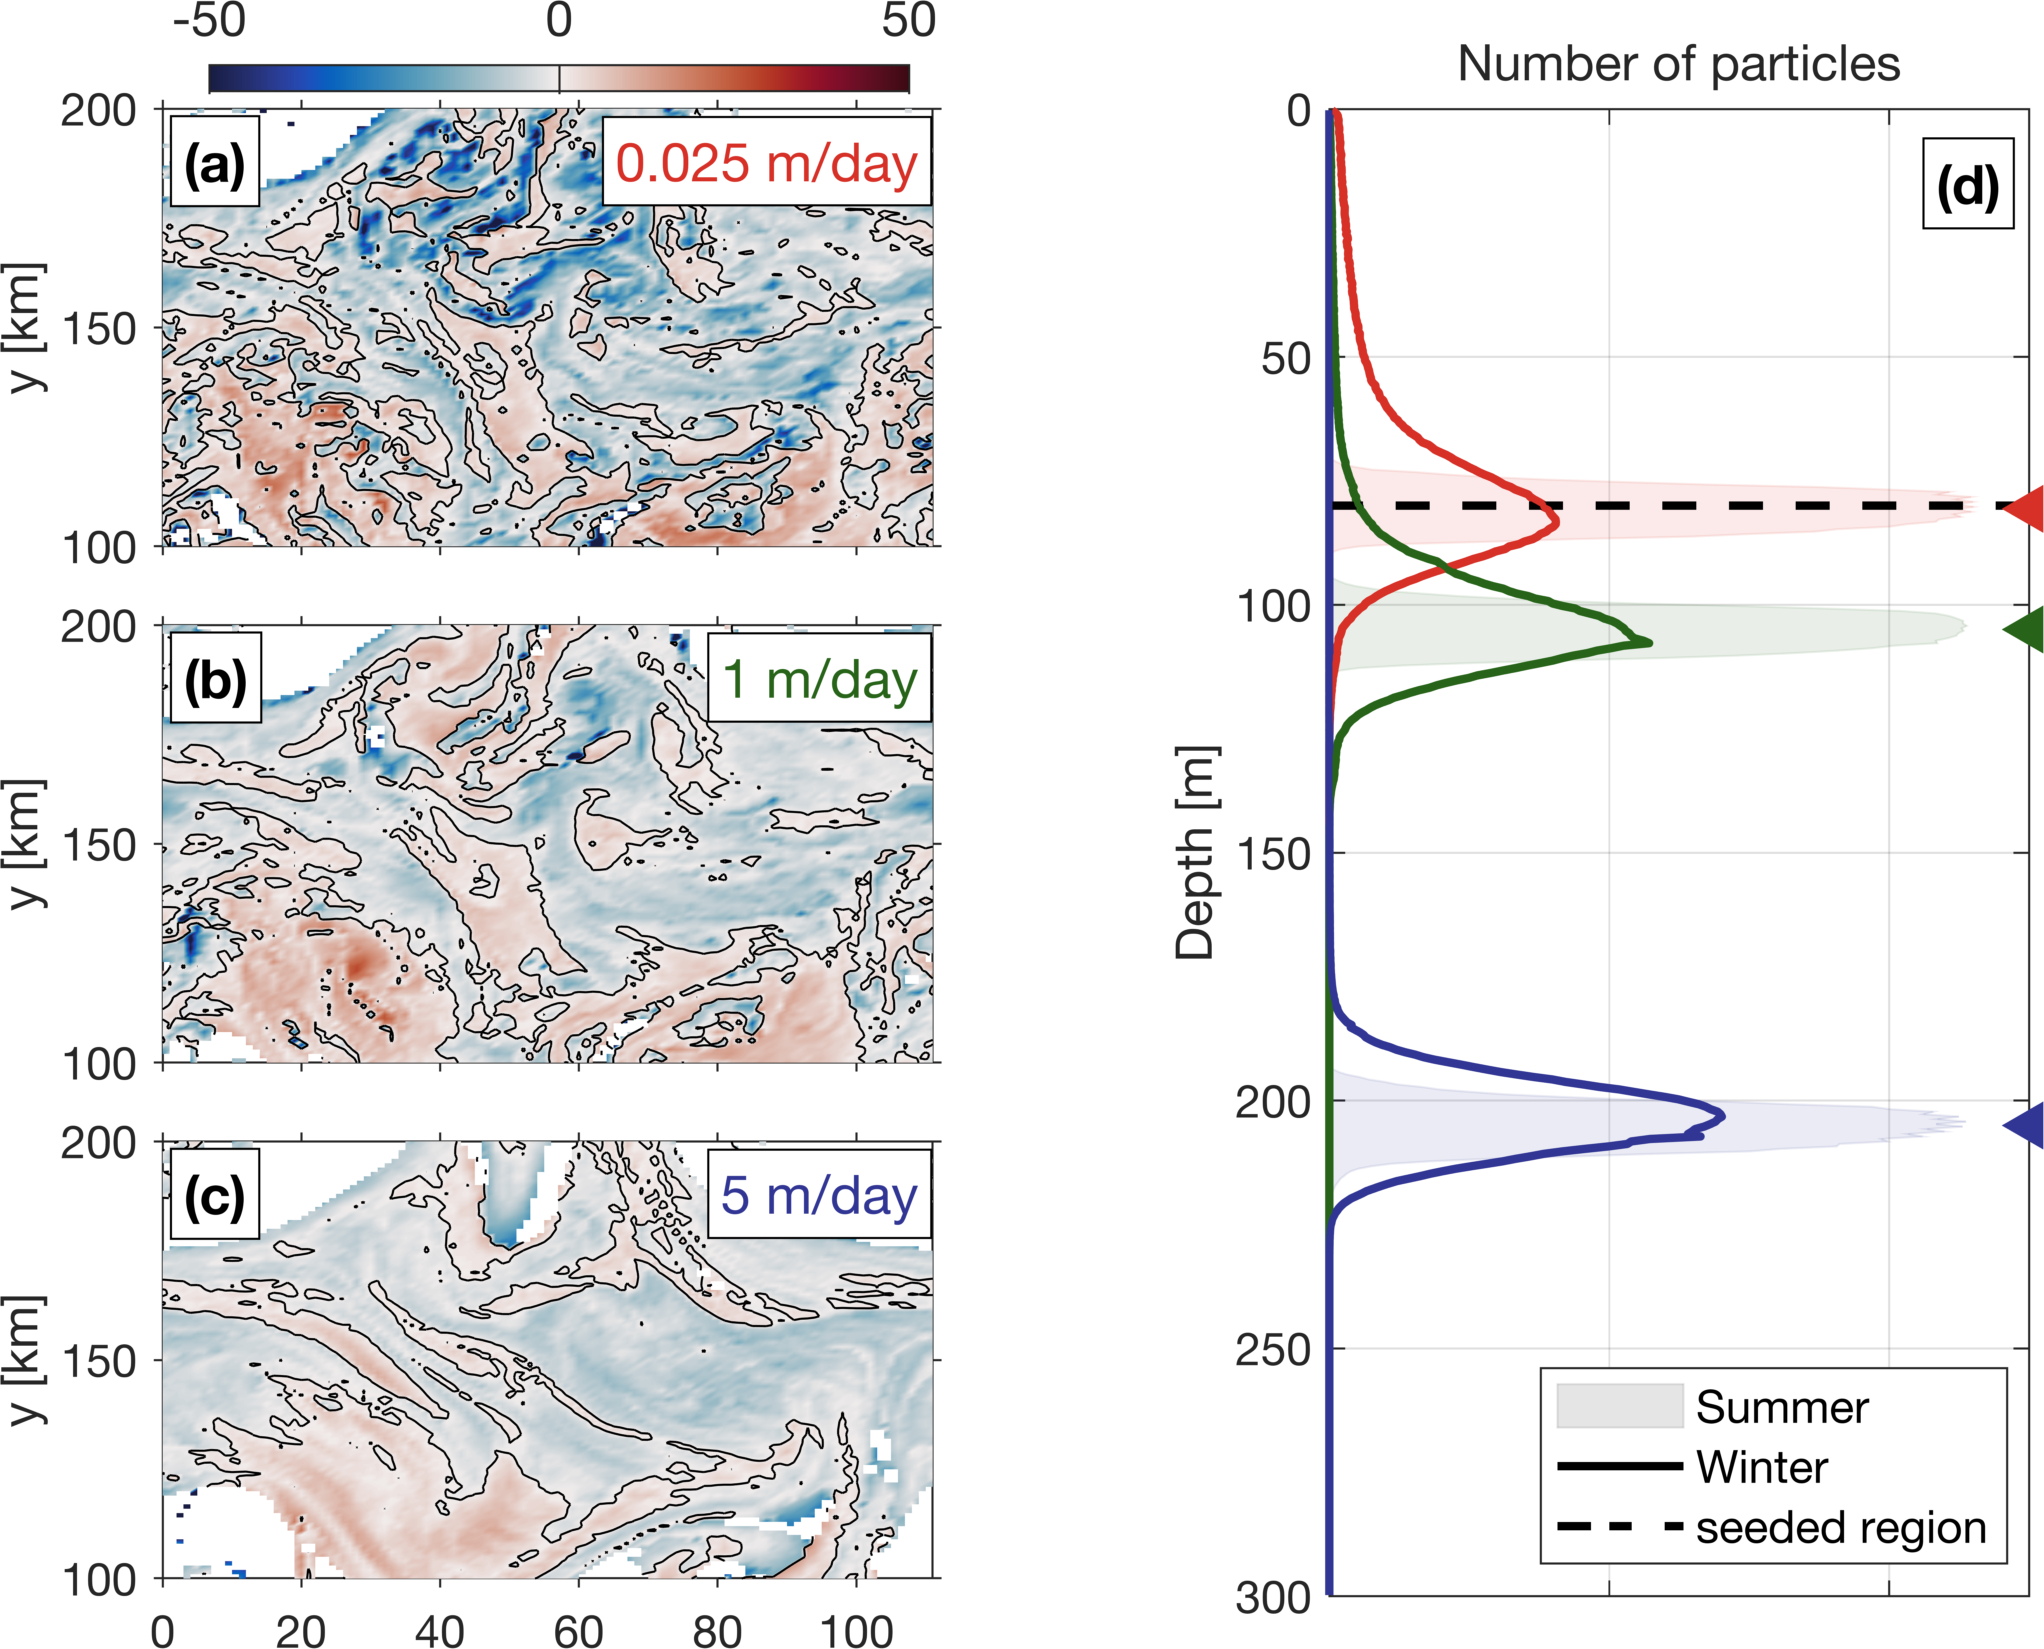
\includegraphics[width = .8\linewidth]{Fig6.png}
		\caption{[left] 
			The median depth anomaly of particles with a sinking speed (a) 0.025 m/d, (b) 1 m/d, (c) 5 m/d within each grid cell for the winter case 25 days after particles are released. The `depth anomaly' is with respect to the `expected' sinking depth (= sinking speed $\times$ time since release). Blue (red) grid cells indicate that the median depth of particles in this cell is deeper (shallower) than expected, based on a 1D gravitational model where $z = w_s\times t$. [right] (d) Probability Distribution Function (PDF) of particles as a function of depth for each velocity class. The winter distribution is shown as thick lines, while the summer distribution is represented by the shaded regions. Triangle markers indicate the expected depth of particles after 25 days based on the 1D gravitational model, which is used as a reference to compute the depth anomalies. Release depth is indicated by the thick dashed line.}	
		\label{fig: particle_depth_distribution}
	\end{figure}
	
	In the winter, however, PDFs of particle density versus depth is wider, in agreement with the stronger vertical ocean currents occurring in the winter (see Figure \ref{fig: dynamics}). A top-view of the deviation in the downward particle flux from the traditionally considered 1D gravitational model can be seen in Figure \ref{fig: particle_depth_distribution} (panels (a)-(c)). Slower-sinking particles deviate more than faster-sinking particles, exhibiting median depth anomalies up to 50 m. This is due to the fact that slower-sinking particles spend more time in the mixed layer, where most of the stronger vertical currents tend to occur (Figure \ref{fig: dynamics}). An interesting result emerges from the spatial distribution of the depth-anomaly: both positive (i.e., particles are shallower than expected) and negative (i.e., particles are deeper than expected) anomalies are organized into features with a length-scale $\mathcal{O}$(1-10 km). This further highlights the importance of winter submesoscale circulation for vertical fluxes of particles.
	
	A relative amount of biomass is associated to the particles using Equation (\ref{eq: biomassjungeslope}). PDFs of relative biomass as a function of the vertical velocity is shown in Figure \ref{fig: biomass_export}. Following the traditional paradigm derived from the simple 1D gravitational model, the downward flux of biomass in the summer is dominated by faster-sinking particle classes capable of carrying particulate material downwards more efficiently. The contribution of slower-sinking particles, however, depends critically on the slope of the size spectrum (see Figure \ref{fig: sinking_velocity_spectrum}). As the Junge slope increases, the spectrum of biomass steepens, and the relative contribution of slower-sinking particles to the downward biomass flux significantly increases (Figure \ref{fig: biomass_export}c). In fact, the contribution of slower-sinking particles to the summer downward flux increases by a factor 100 (from 0.2\% to \change20\%) when the Junge slope varies from $\xi =2$ to $\xi = 4$. While significant, the impact of a change in the Junge slope in summer conditions does not challenge the dominant role played by faster-sinking particles. This result can be explained by the fact that, in the summer, vertical velocities are weak and vertical biomass fluxes are therefore gravitationally-driven ($\left<w_sB\right> > \left<wB\right>$).
	
	%FIG7
	\begin{figure}[t]
		\centering
		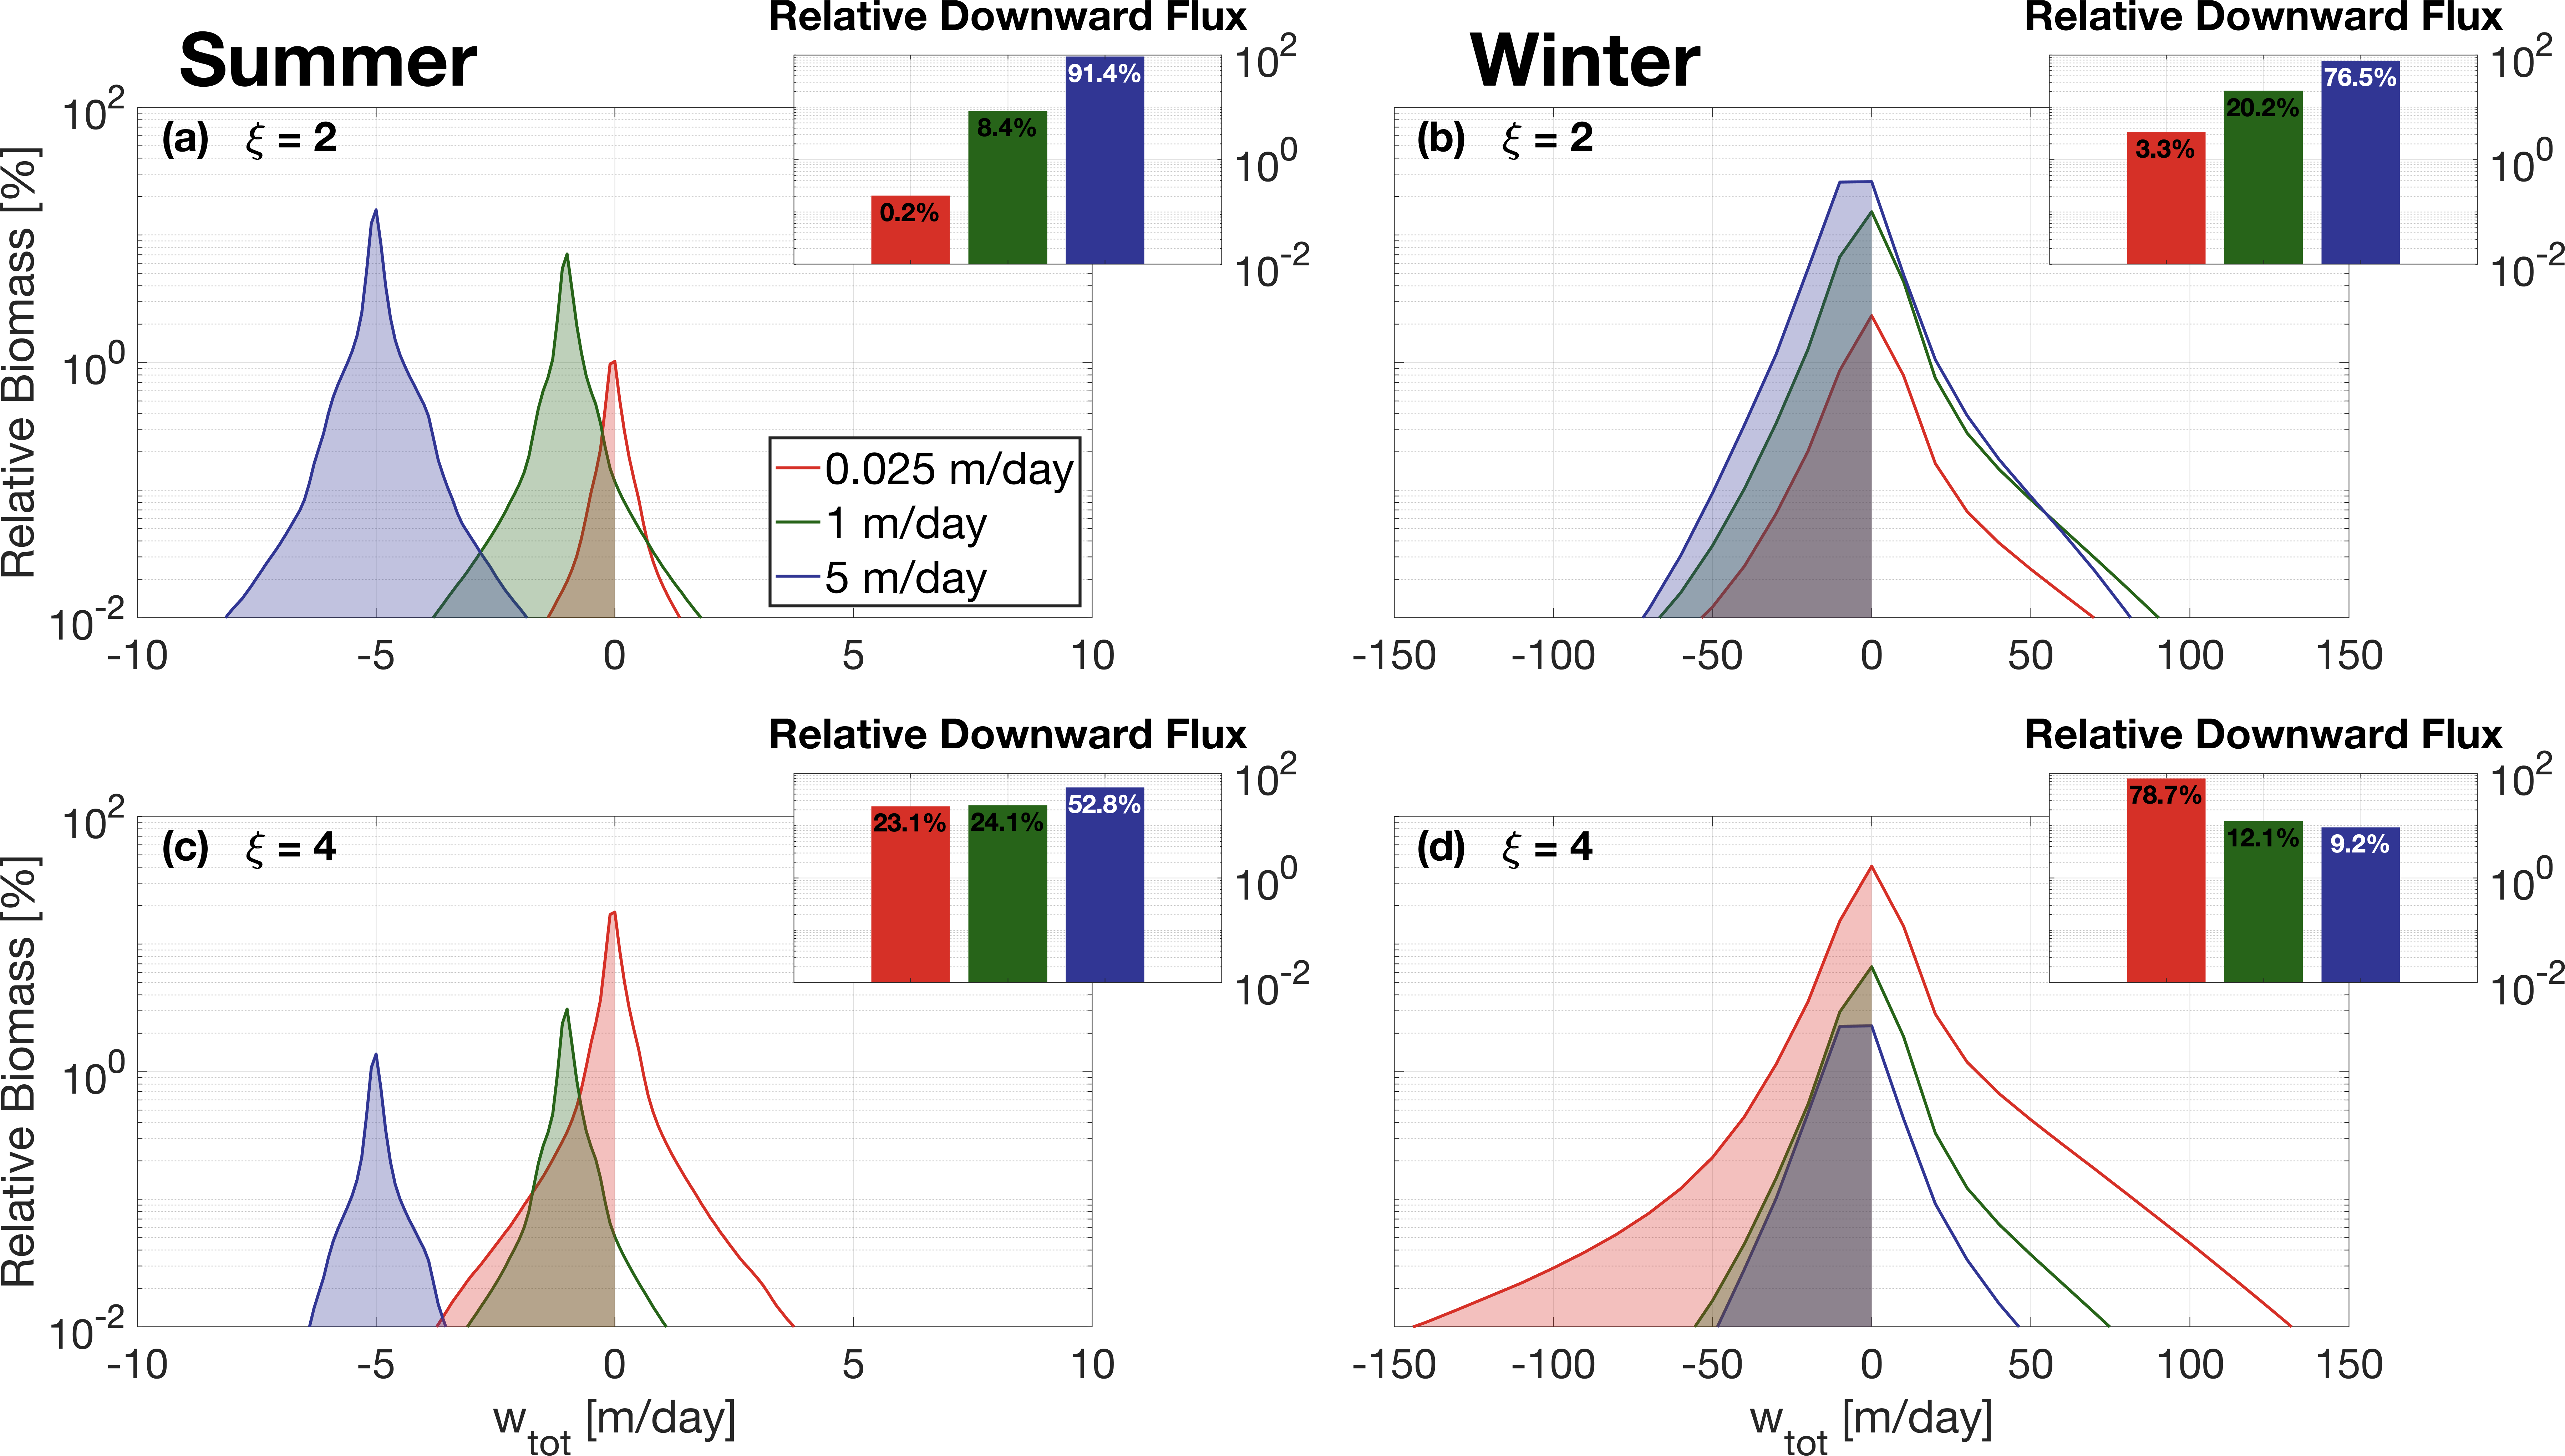
\includegraphics[width = 1\linewidth]{Fig7_revised.png}
		\caption{Probability Distribution Function (PDF) of relative biomass versus total vertical velocity \add{(sinking + advective)} along particle trajectories in the summer case [left] and winter case [right], with a Junge slope of 2 [top] and 4 [bottom]. \add{PDFs are computed from the whole 24-day particle tracking experiments.} Inserts show the integrated relative downward biomass flux associated with each sinking-velocity class, categorized according to their initial sinking velocity. Both winter dynamics and steeper Junge slopes tend to increase the relative contribution of slower-sinking particles.}
		\label{fig: biomass_export}
	\end{figure}
	
	In the winter, PDFs of relative biomass as a function of vertical velocities present a much larger spread, with velocity magnitudes exceeding 50 m/day. For $\xi = 2$, the relative contribution of slower-sinking particles to the downward flux significantly increases from 0.2\% in the summer to about 3\% in the winter, demonstrating the impact advective velocities alone can have on vertical fluxes (Figure \ref{fig: biomass_export}b). Nevertheless, slower-sinking particles remain a relatively small contributor to the total downward flux of biomass. When winter ocean dynamics are coupled with a steeper Junge slope, however, slower-sinking particles largely dominate the downward biomass flux. In our winter simulations with $\xi = 4$, we find that the slowest-sinking particle class is responsible for about 79\% of the biomass flux (Figure \ref{fig: biomass_export}d).
	
	Our results show that both a steepening of the particle size spectrum and the presence of submesoscale dynamics can enhance the contribution of slower-sinking particles to the downward biomass flux. While the former is simply due to an increase in particle density in slower-sinking particle classes, the latter is attributed to the larger vertical velocity generated by submesoscale instabilities. When both are combined, as expected in the wintertime, slower-sinking particles then become the leading contributor to the downward biomass transport. However, slower-sinking particles are generally expected to remineralize on timescales shorter than their export timescale, fueling the argument that the focus should be upon faster-sinking particle classes. The impacts of remineralization on export are thus considered in the following section to test the robustness of the findings.
	
	\subsection{Particle Remineralization}
	\label{sec: results_remin}
	
	Both submesoscale dynamics and the Junge slope were identified as key factors impacting the respective role played by different particle classes in driving downward biomass fluxes. Simple Lagrangian particles were used to isolate the effects of these two factors. In reality, however, sinking velocities of particulate matter varies in time as the particles slowly remineralize. A remineralizing behavior was therefore implemented for the Lagrangian particles, using Equation (\ref{eq: sinking_velocity_remin}), to investigate the impact that remineralization processes have on our findings. The traditional paradigm relies on the fact that slow-sinking particles tend to fully remineralize over short timescales, further enhancing the importance of faster-sinking particles classes in driving downward biomass fluxes. While this paradigm holds for flatter Junge slope, where the biomass content is dominated by faster-sinking particles, it becomes unfit at steeper slopes. 
	
	Figure \ref{fig: biomass_export_remin} compares the relative biomass and downward biomass fluxes associated with each of the modeled particle classes for \add{$\xi = 2$ and} $\xi = 4$ \change{with and without }{including} the remineralization scheme. As previously detailed, downward fluxes of biomass are dominated by faster-sinking particles during summertime and in the absence of remineralization \add{(see Figure} \ref{fig: biomass_export}). This is due to the fact that the flux of biomass $\left<w_{tot}B\right> = \left<w_sB\right> + \left<wB\right>$ is driven by $\left<w_sB\right>$, despite a smaller relative biomass content per particle. This is characteristic of a gravitationally-driven system, where settling velocity dictates the contribution to downward fluxes. Implementing remineralization processes, however, directly affects the particle settling velocity which slows down as particles remineralize. This effect can \add{particularly} be seen in Figure \ref{fig: biomass_export_remin}\add{a and} c, where PDFs of relative biomass per particle class are shifted towards weaker vertical velocities than in the absence of remineralization, as predicted by Equation (\ref{eq: sinking_velocity_remin}). \remove{As a result, the gravitationally-driven term $\left<w_sB\right>$ decreases with time, and the downward flux of biomass becomes generally advectively-driven by day 25 (Figure \ref{fig: biomass_export_remin}).} 

	%FIG8
	\begin{figure}[t!]
		\centering
		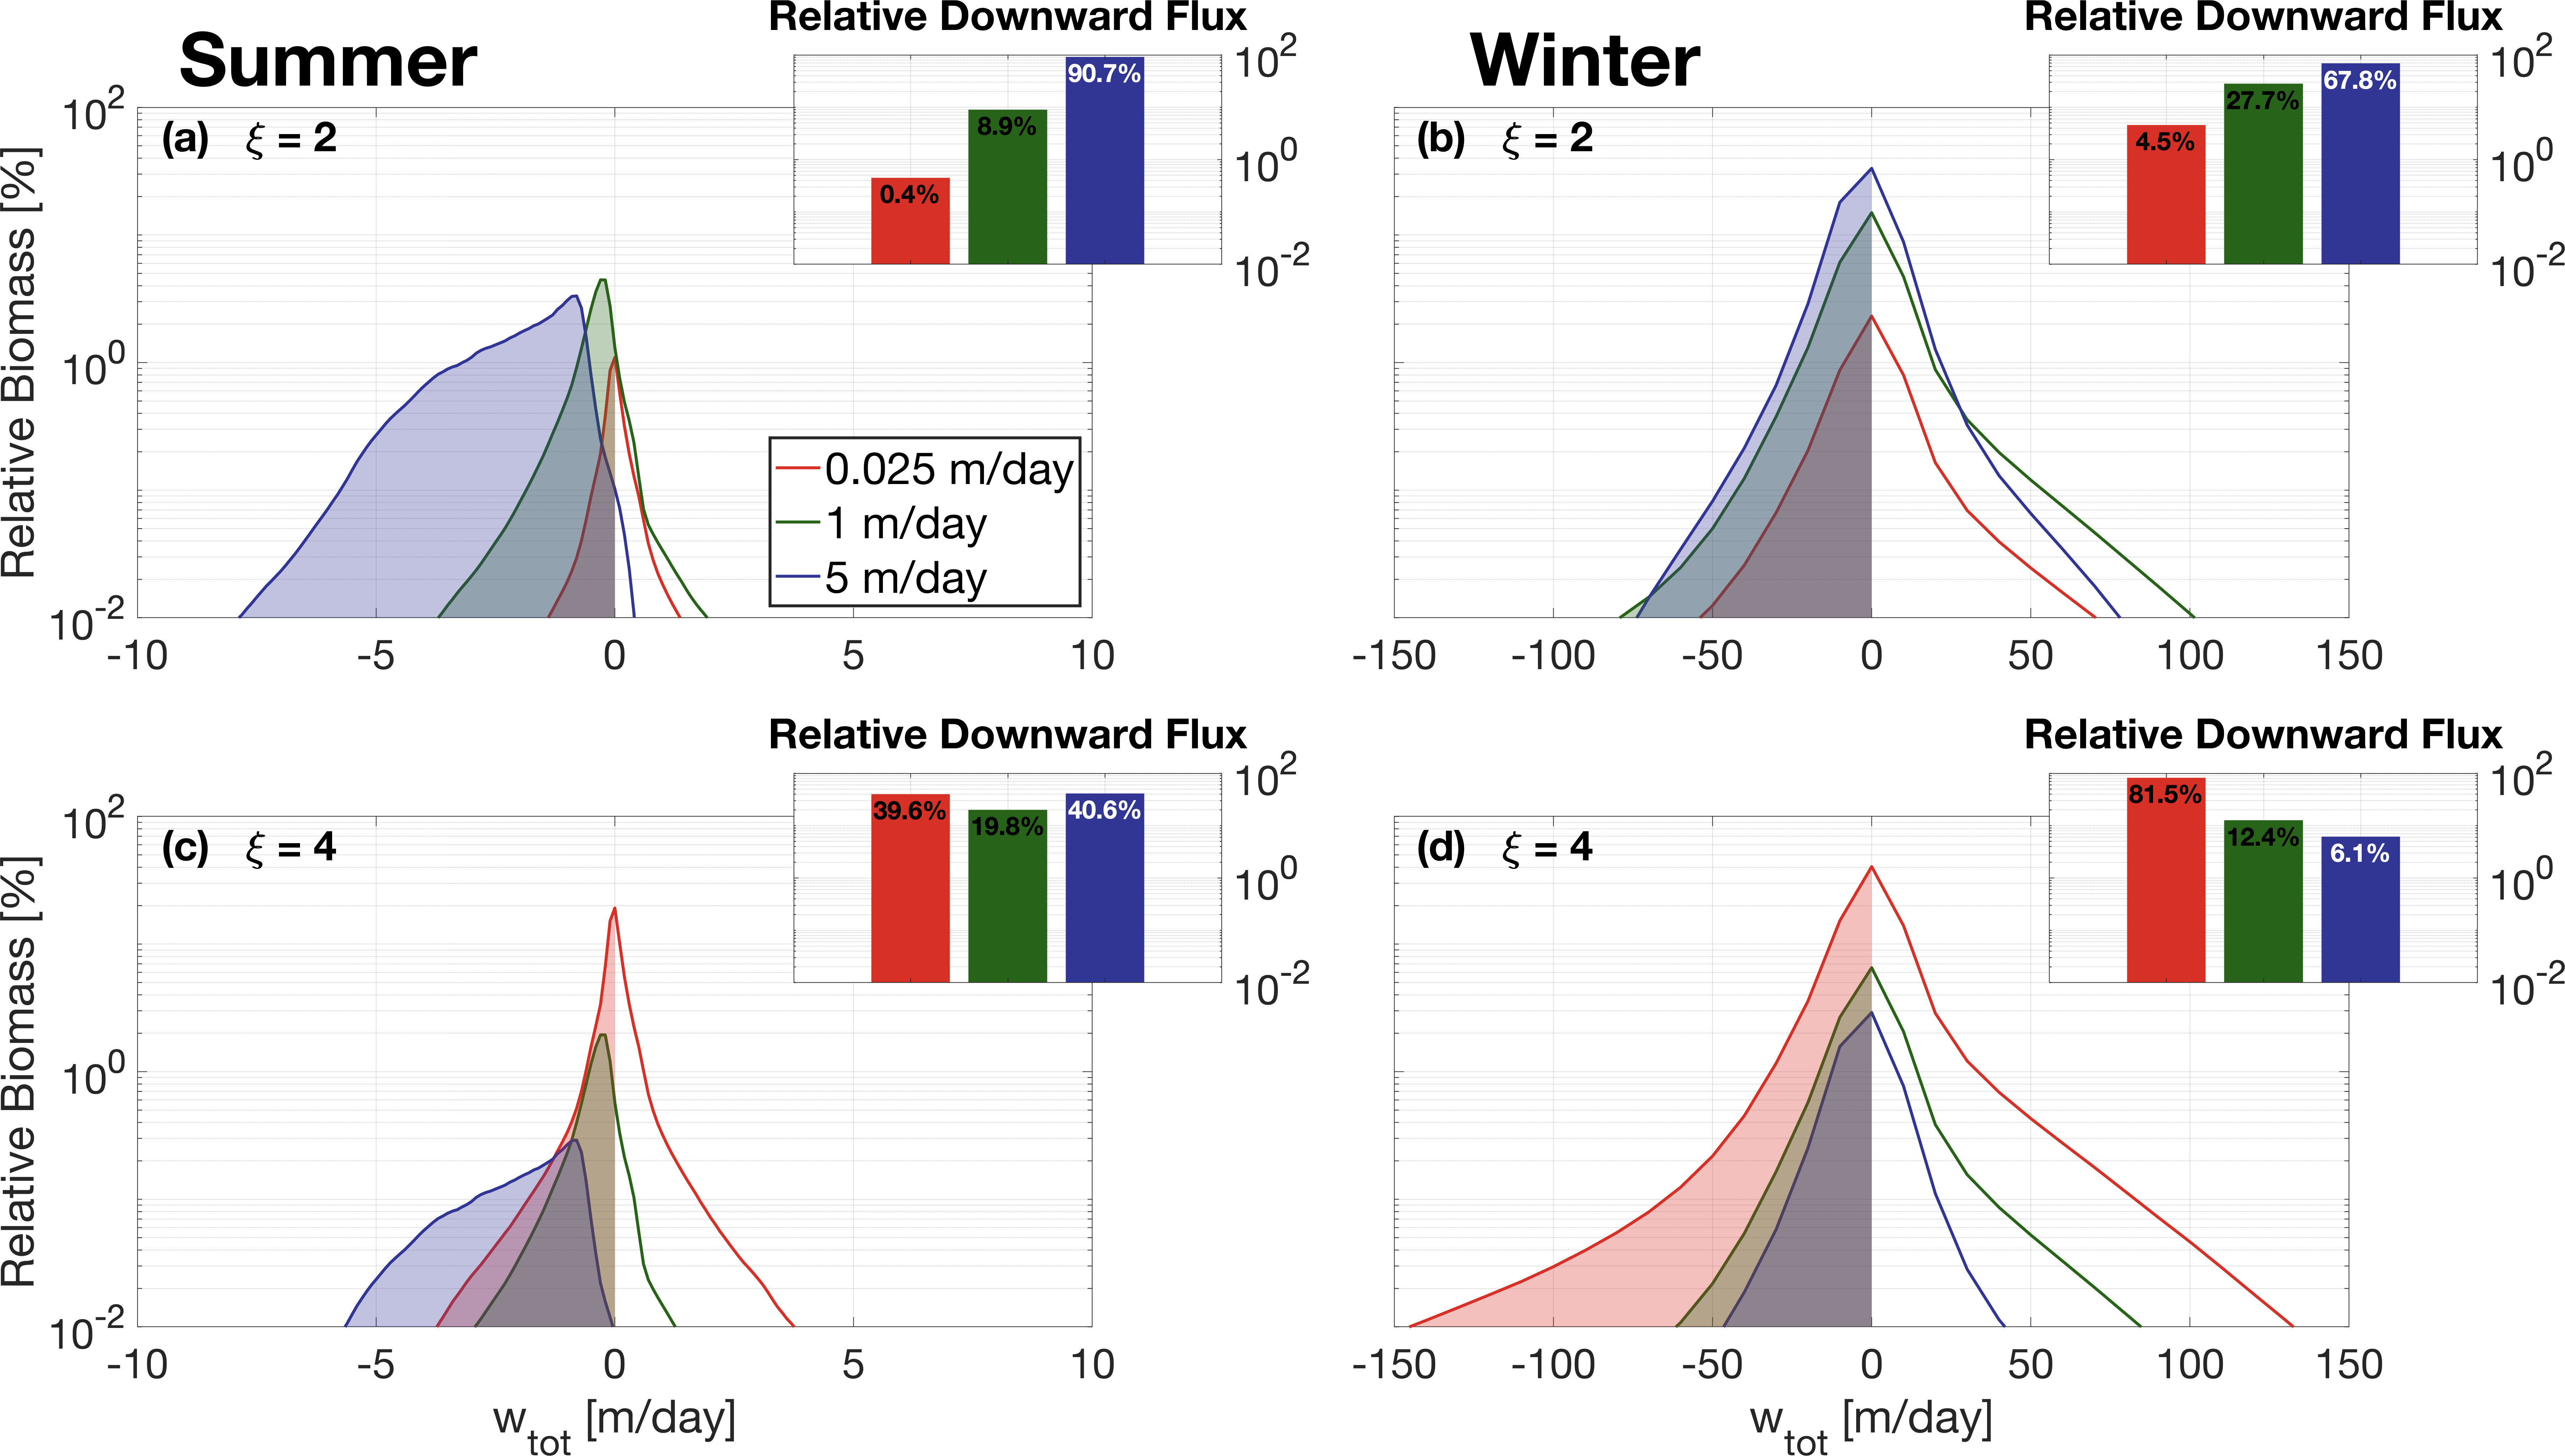
\includegraphics[width = 1\linewidth]{Fig8_revised.png}
		\caption{\change{Probability Distribution Function (PDF) of relative biomass versus total vertical velocity along particle trajectories in the summer case [left] and winter case [right], ignoring [top] and including [bottom] particle remineralization, for $\xi$ = 4 and 25 days after particle release. Inserts show the integrated relative downward biomass flux associated with each sinking-velocity class, categorized according to their initial sinking velocity. Remineralization processes have the greatest impact on fast-sinking particles, especially in summer dynamics.}{Same as Figure \ref{fig: biomass_export}, but including particle remineralization (see Equation \ref{eq: sinking_velocity_remin}).}}	
		\label{fig: biomass_export_remin}
	\end{figure}
	In a advectively-driven system where $\left<w_sB\right> \sim \left<wB\right>$, the relative amount of biomass content in a particle class becomes important and dictates the respective contribution of each particle class to the total downward biomass fluxes. This shift from a gravitationally-driven to an advectively-driven system is observed when implementing particle remineralization in the summer (Figure \ref{fig: biomass_export_remin}\remove{c}): in the absence of remineralization, faster-sinking particles dominate the downward biomass fluxes (\change{60}{53}\%; see Figure \ref{fig: biomass_export}c). When remineralization processes are considered, slower-sinking particles \change{become the dominant contributor}{contribute more} to biomass fluxes (see inset in Figure \ref{fig: biomass_export_remin}c). As shown in Figure \ref{fig: biomass_export}, downward biomass fluxes in the wintertime are generally advectively-driven, due to the larger vertical velocities associated with wintertime ocean dynamics. Biomass fluxes are dominated by the slower-sinking particles \add{when $\xi =4$}, representing 79\% of the downward biomass flux (Figure \ref{fig: biomass_export}d). Even after implementing the remineralization scheme, slower-sinking particles remain the largest contributor to downward biomass fluxes (82\%; see Figure \ref{fig: biomass_export_remin}d).
	
	These results highlight the importance in considering slower-sinking particle classes when considering downward biomass fluxes. It also demonstrates that, contrarily to the traditional paradigm, remineralization processes enhance the role played by slower-sinking particles in biomass fluxes, in cases where the biomass spectrum slope is negative. %The timescales over which the system transitioned from an gravitationally-driven to an advectively-driven system depends on the remineralization model used. 
	
	\section{Discussion}
	\label{sec: Discussion}
	
	\subsection{Dynamical Regimes}
	\label{sec: Discussion_model}
	\textit{Papa\_summer} and \textit{Papa\_winter} experiments were designed to statistically capture the ocean dynamics at Station Papa (145$^o$W, 50$^o$N) in the Northeast Pacific Ocean. After spin-up, the model demonstrated similar distributions of both horizontal ($M^2$) and vertical ($N^2$) density gradients to observational estimates from underwater gliders (see Figures \ref{fig: Papa_summer}, \ref{fig: Papa_winter}, and \ref{fig: dynamics}). The two experiments, however, show significantly different distributions of $M^2$, with the winter distribution exhibiting a longer tail, due to sharper density gradients. The tail of the wintertime distribution is only partially captured by the glider data, due to the fact that underwater gliders sampled gradients at spatial scales of 10 km and greater, while the model has a horizontal resolution of 500~m, allowing sharper submesoscale fronts and filaments to be formed.
	
	Studies investigating submesoscale dynamics traditionally focused on regions where the presence of submesoscale fronts and filaments are established, such as western boundary currents with strong gradients \citep{Dasaro_2011, Thomas_2013}, or the edge of mesoscale features \citep{vanHaren_2006,Waite_2016}. The seasonality in submesoscale dynamics captured in the glider dataset at Station Papa and reflected in the model experiments, echoes the behavior seen from recent observational studies conducted at a similar latitude in the Atlantic Ocean, which demonstrate the intensification of submesoscale dynamics in the wintertime \citep{Thompson_2016, Buckingham_2016}. Despite being sometimes qualified as an ``eddy desert" with low kinetic energy \citep{Chelton_2011}, ocean characteristics in the eastern part of the Pacific subpolar gyre suggest the presence of submesoscale features in the wintertime: strong density gradients, localized Rossby numbers of order 1, a balanced Richardson number $Ri_b = \frac{f^2N^2}{M^4}$ smaller than 1, a positively skewed distribution in vorticity, and a negatively skewed distribution of vertical velocities \citep[see Figure \ref{fig: dynamics};][]{Thomas_2013b,Rudnick_2001, Buckingham_2016}.
	
	Strong downward velocities are hypothesized to enhance POC export by advecting slower-sinking particles out of the mixed layer. \textit{Papa\_winter} indeed exhibits vertical velocities more than 20 times larger than in \textit{Papa\_summer}. The vertical currents in \textit{Papa\_winter}, however, tend to be much patchier than the weaker vertical currents observed in \textit{Papa\_summer}. Because both particle production and downward vertical velocities present a high degree of patchiness, it requires a certain level of covariance between the two fields for the export to effectively be enhanced \citep{Mahadevan_2012}. A more realistic seeding strategy for Lagrangian particles, such as one guided by biological tracers, would likely provide important information towards a better understanding of the effects of patchiness on POC export at submeso-scales
	
	The hypothesis tested in this study is that submesoscale activity enhances export of particulate matter at Station Papa by shortening the export timescale of particulate matter. The wintertime intensification in submesoscale activity has the potential to indeed enhance export (see discussion in Section \ref{sec: discussion_particle}). However, the seasonal cycle in submesoscale activity is out of phase with the one in net community productivity, which peaks in the spring and summertime when the mixed layer is shallower \citep{Plant_2016}. Two mechanisms are therefore present to potentially sustain a year-long POC export flux: In the winter, less particulate material is present in the mixed layer, but active submesoscale dynamics tend to enhance the POC export flux by advecting the more numerous slower-sinking particles into the ocean interior. In the summer, the production of POC is at its yearly maximum, but export tends to be dominated by gravitational sinking, which favors faster-sinking particles and thus exclude part of the particle spectrum from contributing to the export flux.
	
	\subsection{Downward Fluxes}
	\label{sec: discussion_particle}
	
	Analyses of particle tracking experiments reveal that the contribution of slower-sinking particles to the downward particulate flux depends on two main factors: (1) the dynamics of the oceanic flow field, and (2) the slope of the size spectrum (i.e., the Junge slope $\xi$).
	
	Mixed layer ocean dynamics at station Papa change significantly between the winter and the summer. In the winter, submesoscale dynamics are intensified, and sharp fronts and filaments develop in the mixed layer. This seasonal change in dynamics is consistent with recent observations \citep{Thompson_2016, Buckingham_2016}, and models \citep{Brannigan_2015, Callies_2015, Rocha_2016} characterizing the seasonal cycle of submesoscale dynamics. The winter intensification in submesoscale dynamics was proven to have an important impact on the downward flux of all sinking-velocity classes modeled in this experiment.
	
	In the summer,  gravitational sinking governs a downward particulate flux, which is dominated by faster-sinking particles, with little to no contribution from slower-sinking particles. In the winter, however, vertical fluxes tend to be advectively-driven, which leads to a slightly weaker downward flux of faster-sinking particles than in the summer due to resuspension, but a much larger flux of slower-sinking particles, which are present in far greater numbers (Figure \ref{fig: biomass_export}). The gravitationally-driven flux in the summer is mechanistically different from the advectively-driven winter flux, which raises the question as to which process is most efficient in driving a downward flux of particulate material.
	
	In the absence of remineralization, both a steeper size spectrum slope ($\xi>3$ in this case) and enhanced submesoscale dynamics, increase the contribution of slower-sinking particle classes to the downward biomass flux. 
	This is only when both of these conditions are combined, however, that slower-sinking particles dominate the downward flux of biomass (Figure \ref{fig: biomass_export}). 
	This is a significant result, as Junge slopes greater than 3 have been observed in the ocean \add{: In-situ observations yield average spectral slopes varying between 3.5 and 4.5 }\citep[see Table 2 in ]{Kostadinov_2009}\add{, while spectral analysis of satellite data suggest global spectral slopes varying between 3 and 6. More recent observational work located in the Northeast Pacific, including Station Papa, found a spectral slope also greater than 3}\citep[][; Z. Xiaodong, personal communication]{White_2015}.
    \add{Junge slopes are expected to vary in space, depending on the community composition, both lateraly and vertically} \citep{Kostadinov_2009, White_2015}\add{, as well as in time; spectrum slopes tend to be flatter during a spring bloom event, where larger particles (e.g., diatoms) are produced in large quantities, and steeper during the wintertime, when communities are mostly composed of small particles}.
    The threshold value of $\xi =3$ for a change in the biomass spectral slope (see Figure \ref{fig: sinking_velocity_spectrum}b) is of course a consequence of first-order approximations used in this study describing the relationships between particle size, sinking velocity, and biomass content. Nevertheless, our results demonstrate the importance of including the smaller particle size range of the particle spectrum,  in the estimation or measurement of vertical fluxes, especially when submesoscale dynamics are active. It also highlights the importance of better constraining the relationships linking particle size, sinking velocity, and biomass content.
	
	Introducing remineralization processes significantly decreases the biomass flux. Counter-intuitively, however, the implementation of a remineralization scheme further strengthens the contribution of slower-sinking particles to the biomass flux (Figure \ref{fig: biomass_export_remin}). This can be explained by the fact that remineralization processes have a greater impact on sinking-velocity classes that rely on gravitational sinking to be exported, as these particles decelerate as they remineralize. In the summer, all particle classes are similarly affected by remineralization, as downward fluxes are gravitationally-driven. In the winter, however, slower-sinking particles are exported through advective processes. Their export timescale is barely affected by remineralization processes as it only depends on local ocean dynamics.
	
	\add{These results are robust to the range of sinking rates explored. If one considers a particle class with a sinking rate far exceeding the vertical advective velocity }\citep[e.g., 100 m/day; ][]{Turner_2015}\add{, then the associated biomass flux can be estimated by relying on the traditional 1-D paradigm, assuming $w_{tot}\approx w_s$. Combining this approximation with Equation \ref{eq: biomassjungeslope} shows that the slope of the biomass flux spectrum is positive for $\xi<5$, in which case very fast-sinking particles would dominate  vertical biomass fluxes. However, for $\xi>5$, the slope of the biomass flux spectrum becomes negative as well, meaning that the biomass flux is always dominated by the slow-sinking particle classes, regardless of the ocean dynamical regime. While considered large, values of $\xi > 5$ remain realistic and fall within the range obtained from satellite-based estimates} \citep{Kostadinov_2009}.
	
	The results of this study suggest that slow- and non-sinking particles must be considered when studying the downward flux of particulate matter in the upper ocean. The patchiness associated with both particle production and submesoscale features poses a real observational challenge to properly resolve vertical fluxes. Based on our findings, subsequent studies should focus on testing the impact of patchiness on vertical fluxes. In the wintertime, when size spectral slope is steep and submesoscale dynamics most active, vertical fluxes could be grossly underestimated depending on the level of co-occurrence between particle production and stronger vertical currents.
	
	\section{Conclusion}
	\label{sec: Conclusions}
	The main conclusions of this study are: 
	\begin{enumerate}
		\item Ocean dynamics in the subpolar Northeast Pacific exhibit a seasonal cycle with low submesoscale activity in the summertime, and more submesoscale features present in the wintertime. Submesoscale dynamics generate larger, and asymmetric, vertical currents leading to a vertical biomass flux driven by advective processes, as opposed to gravitational sinking in the summertime.
		
		\item Submesoscale dynamics generally enhance the downward particulate flux by increasing the contribution of slower-sinking particles to the total flux through advective transport.   The  slower-sinking particles are found to be significant for export, and can be even make the dominant contribution under certain conditions.
		\item The contribution of slower-sinking particles to the downward biomass flux depends on the slope of the particle size spectra (i.e., the Junge Slope), that controls the relative number of particles per size class. Two cases emerge from this study:
		\begin{enumerate}
			\item If the Junge slope is smaller than 3, larger particles contribute most to vertical biomass fluxes independently of flow dynamics, as there are no mechanisms capable of selectively advecting slower-sinking particles. The system is described as gravitationally-driven.
			\item If the Junge slope is greater than 3, as most commonly observed, ocean dynamics become key for determining which particle classes dominate the downward flux. As submesoscale dynamics become more active, ageostrophic circulations leading to larger vertical velocities develop. In these conditions, downward biomass fluxes are largely driven by the slower-sinking particle classes.
		\end{enumerate}
		\item Remineralization processes logically reduce the amount of biomass flux. However, it unexpectedly enhances the role of slower-sinking particles, which are are advectively transported. The impact of remineralization is greater on faster-sinking particles since it affects both the biomass content and their sinking velocity.
	\end{enumerate}
	
	\section*{Acknowledgments}
	The work was funded by NASA grant NNX16AR48G, to complement the EXport Processes in the global Ocean from RemoTe Sensing (EXPORTS) program. We would like to thank A. Thompson (Caltech) for his useful comments and suggestions, N. Pelland (NOAA) and C. Eriksen (University of Washington) for sharing the glider data collected at Ocean Station Papa, as well as S. Essink for his assistance in developing the particle-tracking code. All data used in this manuscript are publicly available: Ocean Station Papa data is available on PMEL's website \citep[\url{https://www.pmel.noaa.gov/ocs/Papa};][]{PMEL_data} and gridded Argo products can be downloaded at \url{http://www.seanoe.org/data/00348/45945} \citep{Gaillard_2015}. Glider data is archived at the University of Washington's Library \citep[\url{http://hdl.handle.net/1773/41656};][]{Pelland_2018_data}. %Model outputs, and particle trajectories are available on request. % Finally, we are grateful to the two anonymous reviewers for their valuable comments and suggestions.
	
	
	%% ------------------------------------------------------------------------ %%
	%%  REFERENCE LIST AND TEXT CITATIONS
	%\bibliographystyle{apalike}
	\bibliography{sinking_biblio}
	
	
	%% ------------------------------------------------------------------------ %%
	%
	%  END ARTICLE
	%
	%% ------------------------------------------------------------------------ %%
	
	%\end{article}
	%\clearpage
	
	%% ------------------------------------------------------------------------ %%
	%
	%  FIGURES AND TABLES
	%
	%% ------------------------------------------------------------------------ %%
	
\end{document}